% Created by tikzDevice version 0.10.1 on 2017-10-19 13:53:40
% !TEX encoding = UTF-8 Unicode
\begin{tikzpicture}[x=1pt,y=1pt]
\definecolor{fillColor}{RGB}{255,255,255}
\path[use as bounding box,fill=fillColor,fill opacity=0.00] (0,0) rectangle (505.89,505.89);
\begin{scope}
\path[clip] ( 49.20, 61.20) rectangle (480.69,456.69);
\definecolor{fillColor}{RGB}{255,165,0}

\path[fill=fillColor] ( 66.16, 76.83) circle (  1.12);

\path[fill=fillColor] ( 66.16, 76.83) circle (  1.12);

\path[fill=fillColor] ( 67.40, 77.41) circle (  1.12);

\path[fill=fillColor] ( 68.20, 77.64) circle (  1.12);

\path[fill=fillColor] ( 72.99, 82.34) circle (  1.12);

\path[fill=fillColor] ( 76.63, 86.32) circle (  1.12);

\path[fill=fillColor] ( 80.63, 89.50) circle (  1.12);

\path[fill=fillColor] ( 82.41, 86.53) circle (  1.12);

\path[fill=fillColor] ( 82.85, 89.12) circle (  1.12);

\path[fill=fillColor] ( 83.03, 89.83) circle (  1.12);

\path[fill=fillColor] ( 84.36, 93.47) circle (  1.12);

\path[fill=fillColor] ( 84.36, 93.47) circle (  1.12);

\path[fill=fillColor] ( 85.42, 94.80) circle (  1.12);

\path[fill=fillColor] ( 86.93, 96.56) circle (  1.12);

\path[fill=fillColor] ( 89.06, 98.98) circle (  1.12);

\path[fill=fillColor] ( 89.24, 97.81) circle (  1.12);

\path[fill=fillColor] ( 89.86, 97.82) circle (  1.12);

\path[fill=fillColor] ( 90.75,103.69) circle (  1.12);

\path[fill=fillColor] ( 91.55, 97.59) circle (  1.12);

\path[fill=fillColor] ( 92.17,101.34) circle (  1.12);

\path[fill=fillColor] ( 92.26,100.45) circle (  1.12);

\path[fill=fillColor] ( 94.83,105.35) circle (  1.12);

\path[fill=fillColor] ( 96.61,108.40) circle (  1.12);

\path[fill=fillColor] ( 97.85,106.61) circle (  1.12);

\path[fill=fillColor] ( 99.45,101.49) circle (  1.12);

\path[fill=fillColor] (101.14,112.60) circle (  1.12);

\path[fill=fillColor] (101.67,110.50) circle (  1.12);

\path[fill=fillColor] (102.74,114.10) circle (  1.12);

\path[fill=fillColor] (102.91,111.75) circle (  1.12);

\path[fill=fillColor] (108.51,115.16) circle (  1.12);

\path[fill=fillColor] (108.51,115.16) circle (  1.12);

\path[fill=fillColor] (109.13,118.06) circle (  1.12);

\path[fill=fillColor] (109.48,112.88) circle (  1.12);

\path[fill=fillColor] (115.52,115.32) circle (  1.12);

\path[fill=fillColor] (116.32,123.24) circle (  1.12);

\path[fill=fillColor] (121.56,130.77) circle (  1.12);

\path[fill=fillColor] (122.09,116.82) circle (  1.12);

\path[fill=fillColor] (125.38,132.04) circle (  1.12);

\path[fill=fillColor] (127.06,135.64) circle (  1.12);

\path[fill=fillColor] (127.24,143.81) circle (  1.12);

\path[fill=fillColor] (128.40,131.11) circle (  1.12);

\path[fill=fillColor] (129.28,124.03) circle (  1.12);

\path[fill=fillColor] (129.82,140.33) circle (  1.12);

\path[fill=fillColor] (134.61,140.49) circle (  1.12);

\path[fill=fillColor] (137.18,143.96) circle (  1.12);

\path[fill=fillColor] (140.74,141.74) circle (  1.12);

\path[fill=fillColor] (150.68,156.20) circle (  1.12);

\path[fill=fillColor] (151.48,141.45) circle (  1.12);

\path[fill=fillColor] (162.13,171.88) circle (  1.12);

\path[fill=fillColor] (164.62,158.87) circle (  1.12);

\path[fill=fillColor] (176.60,180.34) circle (  1.12);

\path[fill=fillColor] (177.40,176.29) circle (  1.12);

\path[fill=fillColor] (197.82,203.62) circle (  1.12);

\path[fill=fillColor] (210.43,217.75) circle (  1.12);

\path[fill=fillColor] (231.47,227.45) circle (  1.12);

\path[fill=fillColor] (240.00,240.35) circle (  1.12);

\path[fill=fillColor] (248.52,246.91) circle (  1.12);

\path[fill=fillColor] (249.32,248.69) circle (  1.12);

\path[fill=fillColor] (254.56,252.39) circle (  1.12);

\path[fill=fillColor] (299.66,291.49) circle (  1.12);

\path[fill=fillColor] (328.43,314.80) circle (  1.12);

\path[fill=fillColor] (359.23,339.79) circle (  1.12);

\path[fill=fillColor] (380.54,372.93) circle (  1.12);

\path[fill=fillColor] (485.04,462.56) circle (  1.12);
\end{scope}
\begin{scope}
\path[clip] (  0.00,  0.00) rectangle (505.89,505.89);
\definecolor{drawColor}{RGB}{0,0,0}

\path[draw=drawColor,line width= 0.4pt,line join=round,line cap=round] ( 65.18, 61.20) -- (420.32, 61.20);

\path[draw=drawColor,line width= 0.4pt,line join=round,line cap=round] ( 65.18, 61.20) -- ( 65.18, 55.20);

\path[draw=drawColor,line width= 0.4pt,line join=round,line cap=round] (153.97, 61.20) -- (153.97, 55.20);

\path[draw=drawColor,line width= 0.4pt,line join=round,line cap=round] (242.75, 61.20) -- (242.75, 55.20);

\path[draw=drawColor,line width= 0.4pt,line join=round,line cap=round] (331.53, 61.20) -- (331.53, 55.20);

\path[draw=drawColor,line width= 0.4pt,line join=round,line cap=round] (420.32, 61.20) -- (420.32, 55.20);

\node[text=drawColor,anchor=base,inner sep=0pt, outer sep=0pt, scale=  1.00] at ( 65.18, 39.60) {0};

\node[text=drawColor,anchor=base,inner sep=0pt, outer sep=0pt, scale=  1.00] at (153.97, 39.60) {1000};

\node[text=drawColor,anchor=base,inner sep=0pt, outer sep=0pt, scale=  1.00] at (242.75, 39.60) {2000};

\node[text=drawColor,anchor=base,inner sep=0pt, outer sep=0pt, scale=  1.00] at (331.53, 39.60) {3000};

\node[text=drawColor,anchor=base,inner sep=0pt, outer sep=0pt, scale=  1.00] at (420.32, 39.60) {4000};

\path[draw=drawColor,line width= 0.4pt,line join=round,line cap=round] ( 49.20, 75.85) -- ( 49.20,401.35);

\path[draw=drawColor,line width= 0.4pt,line join=round,line cap=round] ( 49.20, 75.85) -- ( 43.20, 75.85);

\path[draw=drawColor,line width= 0.4pt,line join=round,line cap=round] ( 49.20,157.22) -- ( 43.20,157.22);

\path[draw=drawColor,line width= 0.4pt,line join=round,line cap=round] ( 49.20,238.60) -- ( 43.20,238.60);

\path[draw=drawColor,line width= 0.4pt,line join=round,line cap=round] ( 49.20,319.98) -- ( 43.20,319.98);

\path[draw=drawColor,line width= 0.4pt,line join=round,line cap=round] ( 49.20,401.35) -- ( 43.20,401.35);

\node[text=drawColor,rotate= 90.00,anchor=base,inner sep=0pt, outer sep=0pt, scale=  1.00] at ( 34.80, 75.85) {0};

\node[text=drawColor,rotate= 90.00,anchor=base,inner sep=0pt, outer sep=0pt, scale=  1.00] at ( 34.80,157.22) {1000};

\node[text=drawColor,rotate= 90.00,anchor=base,inner sep=0pt, outer sep=0pt, scale=  1.00] at ( 34.80,238.60) {2000};

\node[text=drawColor,rotate= 90.00,anchor=base,inner sep=0pt, outer sep=0pt, scale=  1.00] at ( 34.80,319.98) {3000};

\node[text=drawColor,rotate= 90.00,anchor=base,inner sep=0pt, outer sep=0pt, scale=  1.00] at ( 34.80,401.35) {4000};

\path[draw=drawColor,line width= 0.4pt,line join=round,line cap=round] ( 49.20, 61.20) --
	(480.69, 61.20) --
	(480.69,456.69) --
	( 49.20,456.69) --
	( 49.20, 61.20);
\end{scope}
\begin{scope}
\path[clip] (  0.00,  0.00) rectangle (505.89,505.89);
\definecolor{drawColor}{RGB}{0,0,0}

\node[text=drawColor,anchor=base,inner sep=0pt, outer sep=0pt, scale=  1.00] at (264.94, 15.60) {Actual Sheduling Time};

\node[text=drawColor,rotate= 90.00,anchor=base,inner sep=0pt, outer sep=0pt, scale=  1.00] at ( 10.80,258.94) {Predicted};
\end{scope}
\begin{scope}
\path[clip] ( 49.20, 61.20) rectangle (480.69,456.69);
\definecolor{drawColor}{gray}{0.50}

\path[draw=drawColor,line width= 0.4pt,line join=round,line cap=round] ( 65.18, 75.85) --
	(505.89,479.79);
\end{scope}
\end{tikzpicture}
\begin{tikzpicture}[x=1pt,y=1pt]
\definecolor{fillColor}{RGB}{255,255,255}
\path[use as bounding box,fill=fillColor,fill opacity=0.00] (0,0) rectangle (505.89,505.89);
\begin{scope}
\path[clip] ( 49.20, 61.20) rectangle (480.69,456.69);
\definecolor{drawColor}{RGB}{0,0,255}

\path[draw=drawColor,line width= 0.4pt,line join=round,line cap=round] (280.93,261.51) circle (  2.25);

\path[draw=drawColor,line width= 0.4pt,line join=round,line cap=round] ( 69.98, 79.88) circle (  2.25);

\path[draw=drawColor,line width= 0.4pt,line join=round,line cap=round] (114.72,143.59) circle (  2.25);

\path[draw=drawColor,line width= 0.4pt,line join=round,line cap=round] (324.08,263.34) circle (  2.25);

\path[draw=drawColor,line width= 0.4pt,line join=round,line cap=round] (416.77,362.21) circle (  2.25);

\path[draw=drawColor,line width= 0.4pt,line join=round,line cap=round] (288.92,247.96) circle (  2.25);

\path[draw=drawColor,line width= 0.4pt,line join=round,line cap=round] ( 73.17, 88.30) circle (  2.25);

\path[draw=drawColor,line width= 0.4pt,line join=round,line cap=round] (221.80,294.47) circle (  2.25);

\path[draw=drawColor,line width= 0.4pt,line join=round,line cap=round] ( 69.98, 79.88) circle (  2.25);

\path[draw=drawColor,line width= 0.4pt,line join=round,line cap=round] (311.29,229.28) circle (  2.25);

\path[draw=drawColor,line width= 0.4pt,line join=round,line cap=round] (186.64,165.93) circle (  2.25);

\path[draw=drawColor,line width= 0.4pt,line join=round,line cap=round] (272.94,225.26) circle (  2.25);

\path[draw=drawColor,line width= 0.4pt,line join=round,line cap=round] (407.18,338.41) circle (  2.25);

\path[draw=drawColor,line width= 0.4pt,line join=round,line cap=round] (100.34,104.41) circle (  2.25);

\path[draw=drawColor,line width= 0.4pt,line join=round,line cap=round] (280.93,261.51) circle (  2.25);

\path[draw=drawColor,line width= 0.4pt,line join=round,line cap=round] (159.47,152.02) circle (  2.25);

\path[draw=drawColor,line width= 0.4pt,line join=round,line cap=round] (189.83,199.26) circle (  2.25);

\path[draw=drawColor,line width= 0.4pt,line join=round,line cap=round] (295.31,235.14) circle (  2.25);

\path[draw=drawColor,line width= 0.4pt,line join=round,line cap=round] (359.23,280.18) circle (  2.25);

\path[draw=drawColor,line width= 0.4pt,line join=round,line cap=round] (372.02,284.58) circle (  2.25);

\path[draw=drawColor,line width= 0.4pt,line join=round,line cap=round] (459.91,343.54) circle (  2.25);

\path[draw=drawColor,line width= 0.4pt,line join=round,line cap=round] (122.71,119.06) circle (  2.25);

\path[draw=drawColor,line width= 0.4pt,line join=round,line cap=round] (159.47,152.02) circle (  2.25);

\path[draw=drawColor,line width= 0.4pt,line join=round,line cap=round] (159.47,215.37) circle (  2.25);

\path[draw=drawColor,line width= 0.4pt,line join=round,line cap=round] (263.35,232.58) circle (  2.25);

\path[draw=drawColor,line width= 0.4pt,line join=round,line cap=round] ( 71.57, 85.00) circle (  2.25);

\path[draw=drawColor,line width= 0.4pt,line join=round,line cap=round] (137.10,147.99) circle (  2.25);

\path[draw=drawColor,line width= 0.4pt,line join=round,line cap=round] (218.60,210.97) circle (  2.25);

\path[draw=drawColor,line width= 0.4pt,line join=round,line cap=round] (183.44,214.64) circle (  2.25);

\path[draw=drawColor,line width= 0.4pt,line join=round,line cap=round] (154.68,175.82) circle (  2.25);

\path[draw=drawColor,line width= 0.4pt,line join=round,line cap=round] (189.83,175.09) circle (  2.25);

\path[draw=drawColor,line width= 0.4pt,line join=round,line cap=round] (301.70,289.71) circle (  2.25);

\path[draw=drawColor,line width= 0.4pt,line join=round,line cap=round] (410.37,313.87) circle (  2.25);

\path[draw=drawColor,line width= 0.4pt,line join=round,line cap=round] (106.73,127.48) circle (  2.25);

\path[draw=drawColor,line width= 0.4pt,line join=round,line cap=round] (132.30,150.55) circle (  2.25);

\path[draw=drawColor,line width= 0.4pt,line join=round,line cap=round] (237.78,205.85) circle (  2.25);

\path[draw=drawColor,line width= 0.4pt,line join=round,line cap=round] (395.99,430.32) circle (  2.25);

\path[draw=drawColor,line width= 0.4pt,line join=round,line cap=round] (499.87,376.13) circle (  2.25);

\path[draw=drawColor,line width= 0.4pt,line join=round,line cap=round] (180.25,156.41) circle (  2.25);

\path[draw=drawColor,line width= 0.4pt,line join=round,line cap=round] (370.42,345.37) circle (  2.25);

\path[draw=drawColor,line width= 0.4pt,line join=round,line cap=round] (455.12,325.59) circle (  2.25);

\path[draw=drawColor,line width= 0.4pt,line join=round,line cap=round] (218.60,172.52) circle (  2.25);

\path[draw=drawColor,line width= 0.4pt,line join=round,line cap=round] (186.64,188.27) circle (  2.25);

\path[draw=drawColor,line width= 0.4pt,line join=round,line cap=round] (170.66,186.07) circle (  2.25);

\path[draw=drawColor,line width= 0.4pt,line join=round,line cap=round] (277.73,330.35) circle (  2.25);

\path[draw=drawColor,line width= 0.4pt,line join=round,line cap=round] (218.60,290.44) circle (  2.25);

\path[draw=drawColor,line width= 0.4pt,line join=round,line cap=round] (146.68,173.26) circle (  2.25);
\end{scope}
\begin{scope}
\path[clip] (  0.00,  0.00) rectangle (505.89,505.89);
\definecolor{drawColor}{RGB}{0,0,0}

\path[draw=drawColor,line width= 0.4pt,line join=round,line cap=round] ( 65.18, 61.20) -- (464.71, 61.20);

\path[draw=drawColor,line width= 0.4pt,line join=round,line cap=round] ( 65.18, 61.20) -- ( 65.18, 55.20);

\path[draw=drawColor,line width= 0.4pt,line join=round,line cap=round] (145.09, 61.20) -- (145.09, 55.20);

\path[draw=drawColor,line width= 0.4pt,line join=round,line cap=round] (224.99, 61.20) -- (224.99, 55.20);

\path[draw=drawColor,line width= 0.4pt,line join=round,line cap=round] (304.90, 61.20) -- (304.90, 55.20);

\path[draw=drawColor,line width= 0.4pt,line join=round,line cap=round] (384.80, 61.20) -- (384.80, 55.20);

\path[draw=drawColor,line width= 0.4pt,line join=round,line cap=round] (464.71, 61.20) -- (464.71, 55.20);

\node[text=drawColor,anchor=base,inner sep=0pt, outer sep=0pt, scale=  1.00] at ( 65.18, 39.60) {0};

\node[text=drawColor,anchor=base,inner sep=0pt, outer sep=0pt, scale=  1.00] at (145.09, 39.60) {50};

\node[text=drawColor,anchor=base,inner sep=0pt, outer sep=0pt, scale=  1.00] at (224.99, 39.60) {100};

\node[text=drawColor,anchor=base,inner sep=0pt, outer sep=0pt, scale=  1.00] at (304.90, 39.60) {150};

\node[text=drawColor,anchor=base,inner sep=0pt, outer sep=0pt, scale=  1.00] at (384.80, 39.60) {200};

\node[text=drawColor,anchor=base,inner sep=0pt, outer sep=0pt, scale=  1.00] at (464.71, 39.60) {250};

\path[draw=drawColor,line width= 0.4pt,line join=round,line cap=round] ( 49.20, 75.85) -- ( 49.20,442.04);

\path[draw=drawColor,line width= 0.4pt,line join=round,line cap=round] ( 49.20, 75.85) -- ( 43.20, 75.85);

\path[draw=drawColor,line width= 0.4pt,line join=round,line cap=round] ( 49.20,149.09) -- ( 43.20,149.09);

\path[draw=drawColor,line width= 0.4pt,line join=round,line cap=round] ( 49.20,222.33) -- ( 43.20,222.33);

\path[draw=drawColor,line width= 0.4pt,line join=round,line cap=round] ( 49.20,295.56) -- ( 43.20,295.56);

\path[draw=drawColor,line width= 0.4pt,line join=round,line cap=round] ( 49.20,368.80) -- ( 43.20,368.80);

\path[draw=drawColor,line width= 0.4pt,line join=round,line cap=round] ( 49.20,442.04) -- ( 43.20,442.04);

\node[text=drawColor,rotate= 90.00,anchor=base,inner sep=0pt, outer sep=0pt, scale=  1.00] at ( 34.80, 75.85) {0};

\node[text=drawColor,rotate= 90.00,anchor=base,inner sep=0pt, outer sep=0pt, scale=  1.00] at ( 34.80,149.09) {200};

\node[text=drawColor,rotate= 90.00,anchor=base,inner sep=0pt, outer sep=0pt, scale=  1.00] at ( 34.80,222.33) {400};

\node[text=drawColor,rotate= 90.00,anchor=base,inner sep=0pt, outer sep=0pt, scale=  1.00] at ( 34.80,295.56) {600};

\node[text=drawColor,rotate= 90.00,anchor=base,inner sep=0pt, outer sep=0pt, scale=  1.00] at ( 34.80,368.80) {800};

\node[text=drawColor,rotate= 90.00,anchor=base,inner sep=0pt, outer sep=0pt, scale=  1.00] at ( 34.80,442.04) {1000};

\path[draw=drawColor,line width= 0.4pt,line join=round,line cap=round] ( 49.20, 61.20) --
	(480.69, 61.20) --
	(480.69,456.69) --
	( 49.20,456.69) --
	( 49.20, 61.20);
\end{scope}
\begin{scope}
\path[clip] (  0.00,  0.00) rectangle (505.89,505.89);
\definecolor{drawColor}{RGB}{0,0,0}

\node[text=drawColor,anchor=base,inner sep=0pt, outer sep=0pt, scale=  1.20] at (264.94,477.15) {\bfseries Comparing Schedule length between HEFT heuristics};

\node[text=drawColor,anchor=base,inner sep=0pt, outer sep=0pt, scale=  1.00] at (264.94, 15.60) {Nodes};

\node[text=drawColor,rotate= 90.00,anchor=base,inner sep=0pt, outer sep=0pt, scale=  1.00] at ( 10.80,258.94) {Schedule Length};
\end{scope}
\end{tikzpicture}
) {y};
\end{scope}
\end{tikzpicture}
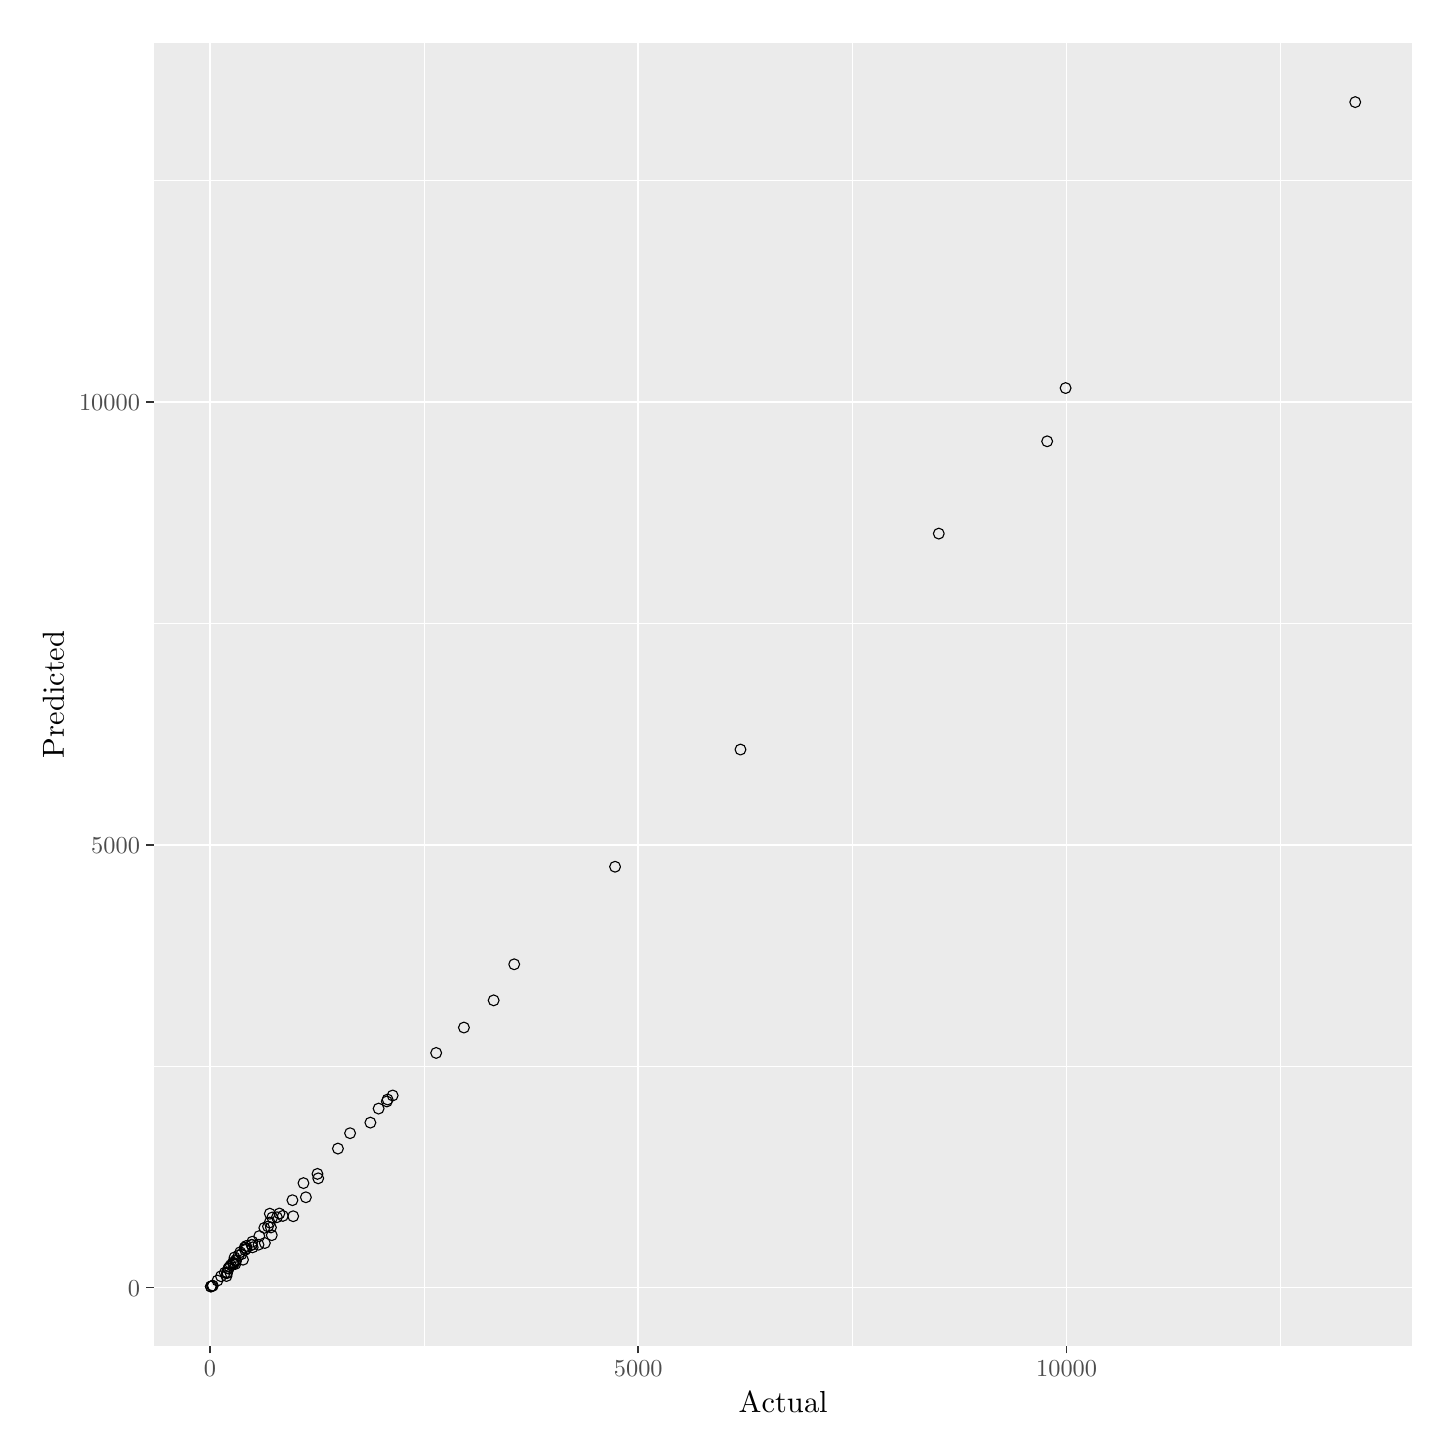
\begin{tikzpicture}[x=1pt,y=1pt]
\definecolor{fillColor}{RGB}{255,255,255}
\path[use as bounding box,fill=fillColor,fill opacity=0.00] (0,0) rectangle (505.89,505.89);
\begin{scope}
\path[clip] (  0.00,  0.00) rectangle (505.89,505.89);
\definecolor{drawColor}{RGB}{255,255,255}
\definecolor{fillColor}{RGB}{255,255,255}

\path[draw=drawColor,line width= 0.6pt,line join=round,line cap=round,fill=fillColor] (  0.00,  0.00) rectangle (505.89,505.89);
\end{scope}
\begin{scope}
\path[clip] ( 45.52, 29.59) rectangle (500.39,500.39);
\definecolor{fillColor}{gray}{0.92}

\path[fill=fillColor] ( 45.52, 29.59) rectangle (500.39,500.39);
\definecolor{drawColor}{RGB}{255,255,255}

\path[draw=drawColor,line width= 0.3pt,line join=round] ( 45.52,130.61) --
	(500.39,130.61);

\path[draw=drawColor,line width= 0.3pt,line join=round] ( 45.52,290.63) --
	(500.39,290.63);

\path[draw=drawColor,line width= 0.3pt,line join=round] ( 45.52,450.66) --
	(500.39,450.66);

\path[draw=drawColor,line width= 0.3pt,line join=round] (143.25, 29.59) --
	(143.25,500.39);

\path[draw=drawColor,line width= 0.3pt,line join=round] (298.03, 29.59) --
	(298.03,500.39);

\path[draw=drawColor,line width= 0.3pt,line join=round] (452.81, 29.59) --
	(452.81,500.39);

\path[draw=drawColor,line width= 0.6pt,line join=round] ( 45.52, 50.60) --
	(500.39, 50.60);

\path[draw=drawColor,line width= 0.6pt,line join=round] ( 45.52,210.62) --
	(500.39,210.62);

\path[draw=drawColor,line width= 0.6pt,line join=round] ( 45.52,370.64) --
	(500.39,370.64);

\path[draw=drawColor,line width= 0.6pt,line join=round] ( 65.86, 29.59) --
	( 65.86,500.39);

\path[draw=drawColor,line width= 0.6pt,line join=round] (220.64, 29.59) --
	(220.64,500.39);

\path[draw=drawColor,line width= 0.6pt,line join=round] (375.42, 29.59) --
	(375.42,500.39);
\definecolor{drawColor}{RGB}{0,0,0}

\path[draw=drawColor,line width= 0.4pt,line join=round,line cap=round] ( 66.20, 50.99) circle (  1.96);

\path[draw=drawColor,line width= 0.4pt,line join=round,line cap=round] ( 66.20, 50.99) circle (  1.96);

\path[draw=drawColor,line width= 0.4pt,line join=round,line cap=round] ( 66.63, 51.22) circle (  1.96);

\path[draw=drawColor,line width= 0.4pt,line join=round,line cap=round] ( 66.91, 51.31) circle (  1.96);

\path[draw=drawColor,line width= 0.4pt,line join=round,line cap=round] ( 68.58, 53.15) circle (  1.96);

\path[draw=drawColor,line width= 0.4pt,line join=round,line cap=round] ( 69.85, 54.72) circle (  1.96);

\path[draw=drawColor,line width= 0.4pt,line join=round,line cap=round] ( 71.24, 55.97) circle (  1.96);

\path[draw=drawColor,line width= 0.4pt,line join=round,line cap=round] ( 71.86, 54.80) circle (  1.96);

\path[draw=drawColor,line width= 0.4pt,line join=round,line cap=round] ( 72.02, 55.82) circle (  1.96);

\path[draw=drawColor,line width= 0.4pt,line join=round,line cap=round] ( 72.08, 56.10) circle (  1.96);

\path[draw=drawColor,line width= 0.4pt,line join=round,line cap=round] ( 72.54, 57.53) circle (  1.96);

\path[draw=drawColor,line width= 0.4pt,line join=round,line cap=round] ( 72.54, 57.53) circle (  1.96);

\path[draw=drawColor,line width= 0.4pt,line join=round,line cap=round] ( 72.91, 58.06) circle (  1.96);

\path[draw=drawColor,line width= 0.4pt,line join=round,line cap=round] ( 73.44, 58.75) circle (  1.96);

\path[draw=drawColor,line width= 0.4pt,line join=round,line cap=round] ( 74.18, 59.70) circle (  1.96);

\path[draw=drawColor,line width= 0.4pt,line join=round,line cap=round] ( 74.25, 59.24) circle (  1.96);

\path[draw=drawColor,line width= 0.4pt,line join=round,line cap=round] ( 74.46, 59.24) circle (  1.96);

\path[draw=drawColor,line width= 0.4pt,line join=round,line cap=round] ( 74.77, 61.55) circle (  1.96);

\path[draw=drawColor,line width= 0.4pt,line join=round,line cap=round] ( 75.05, 59.15) circle (  1.96);

\path[draw=drawColor,line width= 0.4pt,line join=round,line cap=round] ( 75.27, 60.63) circle (  1.96);

\path[draw=drawColor,line width= 0.4pt,line join=round,line cap=round] ( 75.30, 60.28) circle (  1.96);

\path[draw=drawColor,line width= 0.4pt,line join=round,line cap=round] ( 76.20, 62.20) circle (  1.96);

\path[draw=drawColor,line width= 0.4pt,line join=round,line cap=round] ( 76.81, 63.40) circle (  1.96);

\path[draw=drawColor,line width= 0.4pt,line join=round,line cap=round] ( 77.25, 62.70) circle (  1.96);

\path[draw=drawColor,line width= 0.4pt,line join=round,line cap=round] ( 77.81, 60.69) circle (  1.96);

\path[draw=drawColor,line width= 0.4pt,line join=round,line cap=round] ( 78.39, 65.06) circle (  1.96);

\path[draw=drawColor,line width= 0.4pt,line join=round,line cap=round] ( 78.58, 64.23) circle (  1.96);

\path[draw=drawColor,line width= 0.4pt,line join=round,line cap=round] ( 78.95, 65.65) circle (  1.96);

\path[draw=drawColor,line width= 0.4pt,line join=round,line cap=round] ( 79.01, 64.72) circle (  1.96);

\path[draw=drawColor,line width= 0.4pt,line join=round,line cap=round] ( 80.96, 66.06) circle (  1.96);

\path[draw=drawColor,line width= 0.4pt,line join=round,line cap=round] ( 80.96, 66.06) circle (  1.96);

\path[draw=drawColor,line width= 0.4pt,line join=round,line cap=round] ( 81.18, 67.20) circle (  1.96);

\path[draw=drawColor,line width= 0.4pt,line join=round,line cap=round] ( 81.30, 65.17) circle (  1.96);

\path[draw=drawColor,line width= 0.4pt,line join=round,line cap=round] ( 83.41, 66.12) circle (  1.96);

\path[draw=drawColor,line width= 0.4pt,line join=round,line cap=round] ( 83.69, 69.24) circle (  1.96);

\path[draw=drawColor,line width= 0.4pt,line join=round,line cap=round] ( 85.51, 72.20) circle (  1.96);

\path[draw=drawColor,line width= 0.4pt,line join=round,line cap=round] ( 85.70, 66.72) circle (  1.96);

\path[draw=drawColor,line width= 0.4pt,line join=round,line cap=round] ( 86.84, 72.70) circle (  1.96);

\path[draw=drawColor,line width= 0.4pt,line join=round,line cap=round] ( 87.43, 74.12) circle (  1.96);

\path[draw=drawColor,line width= 0.4pt,line join=round,line cap=round] ( 87.49, 77.33) circle (  1.96);

\path[draw=drawColor,line width= 0.4pt,line join=round,line cap=round] ( 87.90, 72.34) circle (  1.96);

\path[draw=drawColor,line width= 0.4pt,line join=round,line cap=round] ( 88.21, 69.55) circle (  1.96);

\path[draw=drawColor,line width= 0.4pt,line join=round,line cap=round] ( 88.39, 75.96) circle (  1.96);

\path[draw=drawColor,line width= 0.4pt,line join=round,line cap=round] ( 90.06, 76.03) circle (  1.96);

\path[draw=drawColor,line width= 0.4pt,line join=round,line cap=round] ( 90.96, 77.39) circle (  1.96);

\path[draw=drawColor,line width= 0.4pt,line join=round,line cap=round] ( 92.20, 76.52) circle (  1.96);

\path[draw=drawColor,line width= 0.4pt,line join=round,line cap=round] ( 95.67, 82.20) circle (  1.96);

\path[draw=drawColor,line width= 0.4pt,line join=round,line cap=round] ( 95.95, 76.40) circle (  1.96);

\path[draw=drawColor,line width= 0.4pt,line join=round,line cap=round] ( 99.66, 88.37) circle (  1.96);

\path[draw=drawColor,line width= 0.4pt,line join=round,line cap=round] (100.53, 83.25) circle (  1.96);

\path[draw=drawColor,line width= 0.4pt,line join=round,line cap=round] (104.71, 91.70) circle (  1.96);

\path[draw=drawColor,line width= 0.4pt,line join=round,line cap=round] (104.99, 90.10) circle (  1.96);

\path[draw=drawColor,line width= 0.4pt,line join=round,line cap=round] (112.11,100.85) circle (  1.96);

\path[draw=drawColor,line width= 0.4pt,line join=round,line cap=round] (116.50,106.41) circle (  1.96);

\path[draw=drawColor,line width= 0.4pt,line join=round,line cap=round] (123.84,110.23) circle (  1.96);

\path[draw=drawColor,line width= 0.4pt,line join=round,line cap=round] (126.81,115.30) circle (  1.96);

\path[draw=drawColor,line width= 0.4pt,line join=round,line cap=round] (129.78,117.88) circle (  1.96);

\path[draw=drawColor,line width= 0.4pt,line join=round,line cap=round] (130.06,118.58) circle (  1.96);

\path[draw=drawColor,line width= 0.4pt,line join=round,line cap=round] (131.89,120.03) circle (  1.96);

\path[draw=drawColor,line width= 0.4pt,line join=round,line cap=round] (147.61,135.41) circle (  1.96);

\path[draw=drawColor,line width= 0.4pt,line join=round,line cap=round] (157.64,144.58) circle (  1.96);

\path[draw=drawColor,line width= 0.4pt,line join=round,line cap=round] (168.38,154.41) circle (  1.96);

\path[draw=drawColor,line width= 0.4pt,line join=round,line cap=round] (175.81,167.44) circle (  1.96);

\path[draw=drawColor,line width= 0.4pt,line join=round,line cap=round] (212.25,202.69) circle (  1.96);

\path[draw=drawColor,line width= 0.4pt,line join=round,line cap=round] (257.57,245.04) circle (  1.96);

\path[draw=drawColor,line width= 0.4pt,line join=round,line cap=round] (329.23,323.07) circle (  1.96);

\path[draw=drawColor,line width= 0.4pt,line join=round,line cap=round] (368.39,356.42) circle (  1.96);

\path[draw=drawColor,line width= 0.4pt,line join=round,line cap=round] (375.05,375.66) circle (  1.96);

\path[draw=drawColor,line width= 0.4pt,line join=round,line cap=round] (479.71,478.99) circle (  1.96);
\end{scope}
\begin{scope}
\path[clip] (  0.00,  0.00) rectangle (505.89,505.89);
\definecolor{drawColor}{gray}{0.30}

\node[text=drawColor,anchor=base east,inner sep=0pt, outer sep=0pt, scale=  0.88] at ( 40.57, 47.57) {0};

\node[text=drawColor,anchor=base east,inner sep=0pt, outer sep=0pt, scale=  0.88] at ( 40.57,207.59) {5000};

\node[text=drawColor,anchor=base east,inner sep=0pt, outer sep=0pt, scale=  0.88] at ( 40.57,367.61) {10000};
\end{scope}
\begin{scope}
\path[clip] (  0.00,  0.00) rectangle (505.89,505.89);
\definecolor{drawColor}{gray}{0.20}

\path[draw=drawColor,line width= 0.6pt,line join=round] ( 42.77, 50.60) --
	( 45.52, 50.60);

\path[draw=drawColor,line width= 0.6pt,line join=round] ( 42.77,210.62) --
	( 45.52,210.62);

\path[draw=drawColor,line width= 0.6pt,line join=round] ( 42.77,370.64) --
	( 45.52,370.64);
\end{scope}
\begin{scope}
\path[clip] (  0.00,  0.00) rectangle (505.89,505.89);
\definecolor{drawColor}{gray}{0.20}

\path[draw=drawColor,line width= 0.6pt,line join=round] ( 65.86, 26.84) --
	( 65.86, 29.59);

\path[draw=drawColor,line width= 0.6pt,line join=round] (220.64, 26.84) --
	(220.64, 29.59);

\path[draw=drawColor,line width= 0.6pt,line join=round] (375.42, 26.84) --
	(375.42, 29.59);
\end{scope}
\begin{scope}
\path[clip] (  0.00,  0.00) rectangle (505.89,505.89);
\definecolor{drawColor}{gray}{0.30}

\node[text=drawColor,anchor=base,inner sep=0pt, outer sep=0pt, scale=  0.88] at ( 65.86, 18.58) {0};

\node[text=drawColor,anchor=base,inner sep=0pt, outer sep=0pt, scale=  0.88] at (220.64, 18.58) {5000};

\node[text=drawColor,anchor=base,inner sep=0pt, outer sep=0pt, scale=  0.88] at (375.42, 18.58) {10000};
\end{scope}
\begin{scope}
\path[clip] (  0.00,  0.00) rectangle (505.89,505.89);
\definecolor{drawColor}{RGB}{0,0,0}

\node[text=drawColor,anchor=base,inner sep=0pt, outer sep=0pt, scale=  1.10] at (272.96,  5.50) {Actual};
\end{scope}
\begin{scope}
\path[clip] (  0.00,  0.00) rectangle (505.89,505.89);
\definecolor{drawColor}{RGB}{0,0,0}

\node[text=drawColor,rotate= 90.00,anchor=base,inner sep=0pt, outer sep=0pt, scale=  1.10] at ( 13.08,264.99) {Predicted};
\end{scope}
\end{tikzpicture}
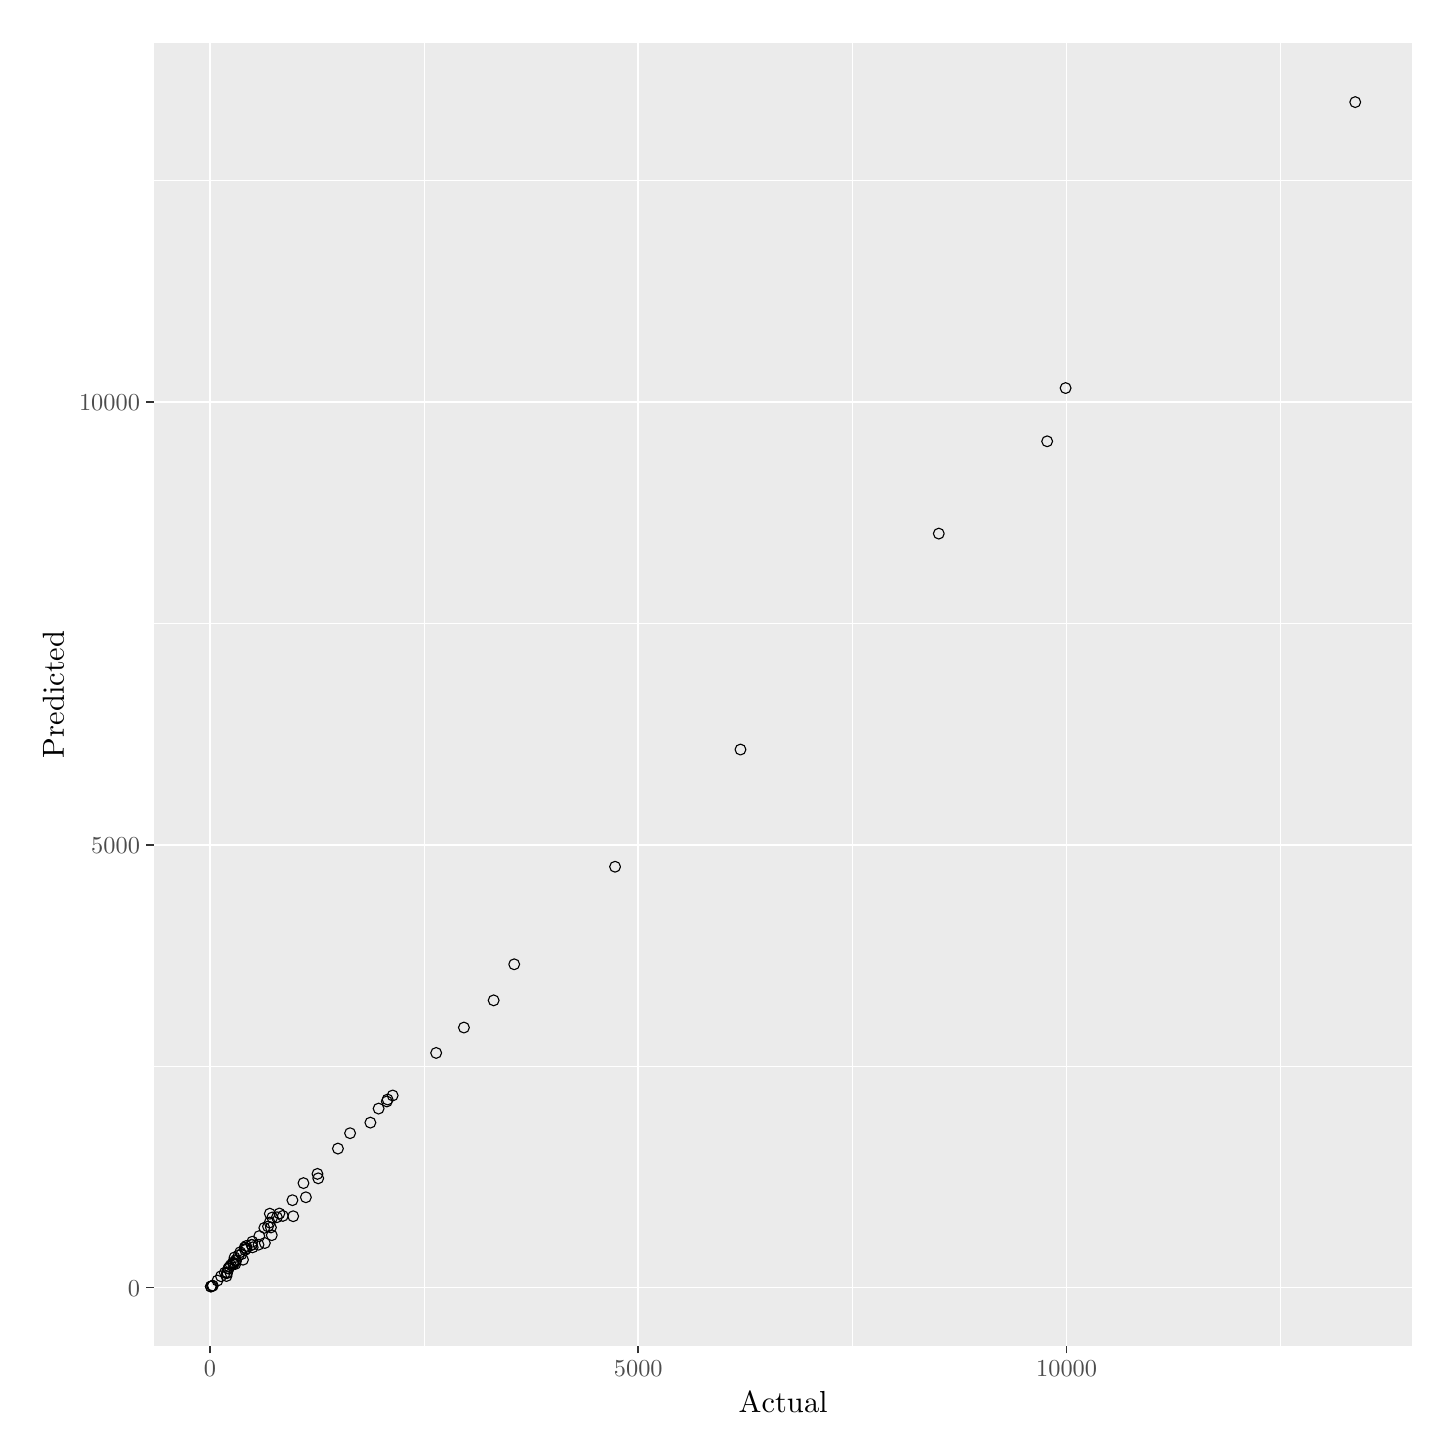
\begin{tikzpicture}[x=1pt,y=1pt]
\definecolor{fillColor}{RGB}{255,255,255}
\path[use as bounding box,fill=fillColor,fill opacity=0.00] (0,0) rectangle (505.89,505.89);
\begin{scope}
\path[clip] (  0.00,  0.00) rectangle (505.89,505.89);
\definecolor{drawColor}{RGB}{255,255,255}
\definecolor{fillColor}{RGB}{255,255,255}

\path[draw=drawColor,line width= 0.6pt,line join=round,line cap=round,fill=fillColor] (  0.00,  0.00) rectangle (505.89,505.89);
\end{scope}
\begin{scope}
\path[clip] ( 45.52, 29.59) rectangle (500.39,500.39);
\definecolor{fillColor}{gray}{0.92}

\path[fill=fillColor] ( 45.52, 29.59) rectangle (500.39,500.39);
\definecolor{drawColor}{RGB}{255,255,255}

\path[draw=drawColor,line width= 0.3pt,line join=round] ( 45.52,130.61) --
	(500.39,130.61);

\path[draw=drawColor,line width= 0.3pt,line join=round] ( 45.52,290.63) --
	(500.39,290.63);

\path[draw=drawColor,line width= 0.3pt,line join=round] ( 45.52,450.66) --
	(500.39,450.66);

\path[draw=drawColor,line width= 0.3pt,line join=round] (143.25, 29.59) --
	(143.25,500.39);

\path[draw=drawColor,line width= 0.3pt,line join=round] (298.03, 29.59) --
	(298.03,500.39);

\path[draw=drawColor,line width= 0.3pt,line join=round] (452.81, 29.59) --
	(452.81,500.39);

\path[draw=drawColor,line width= 0.6pt,line join=round] ( 45.52, 50.60) --
	(500.39, 50.60);

\path[draw=drawColor,line width= 0.6pt,line join=round] ( 45.52,210.62) --
	(500.39,210.62);

\path[draw=drawColor,line width= 0.6pt,line join=round] ( 45.52,370.64) --
	(500.39,370.64);

\path[draw=drawColor,line width= 0.6pt,line join=round] ( 65.86, 29.59) --
	( 65.86,500.39);

\path[draw=drawColor,line width= 0.6pt,line join=round] (220.64, 29.59) --
	(220.64,500.39);

\path[draw=drawColor,line width= 0.6pt,line join=round] (375.42, 29.59) --
	(375.42,500.39);
\definecolor{drawColor}{RGB}{0,0,0}

\path[draw=drawColor,line width= 0.4pt,line join=round,line cap=round] ( 66.20, 50.99) circle (  1.96);

\path[draw=drawColor,line width= 0.4pt,line join=round,line cap=round] ( 66.20, 50.99) circle (  1.96);

\path[draw=drawColor,line width= 0.4pt,line join=round,line cap=round] ( 66.63, 51.22) circle (  1.96);

\path[draw=drawColor,line width= 0.4pt,line join=round,line cap=round] ( 66.91, 51.31) circle (  1.96);

\path[draw=drawColor,line width= 0.4pt,line join=round,line cap=round] ( 68.58, 53.15) circle (  1.96);

\path[draw=drawColor,line width= 0.4pt,line join=round,line cap=round] ( 69.85, 54.72) circle (  1.96);

\path[draw=drawColor,line width= 0.4pt,line join=round,line cap=round] ( 71.24, 55.97) circle (  1.96);

\path[draw=drawColor,line width= 0.4pt,line join=round,line cap=round] ( 71.86, 54.80) circle (  1.96);

\path[draw=drawColor,line width= 0.4pt,line join=round,line cap=round] ( 72.02, 55.82) circle (  1.96);

\path[draw=drawColor,line width= 0.4pt,line join=round,line cap=round] ( 72.08, 56.10) circle (  1.96);

\path[draw=drawColor,line width= 0.4pt,line join=round,line cap=round] ( 72.54, 57.53) circle (  1.96);

\path[draw=drawColor,line width= 0.4pt,line join=round,line cap=round] ( 72.54, 57.53) circle (  1.96);

\path[draw=drawColor,line width= 0.4pt,line join=round,line cap=round] ( 72.91, 58.06) circle (  1.96);

\path[draw=drawColor,line width= 0.4pt,line join=round,line cap=round] ( 73.44, 58.75) circle (  1.96);

\path[draw=drawColor,line width= 0.4pt,line join=round,line cap=round] ( 74.18, 59.70) circle (  1.96);

\path[draw=drawColor,line width= 0.4pt,line join=round,line cap=round] ( 74.25, 59.24) circle (  1.96);

\path[draw=drawColor,line width= 0.4pt,line join=round,line cap=round] ( 74.46, 59.24) circle (  1.96);

\path[draw=drawColor,line width= 0.4pt,line join=round,line cap=round] ( 74.77, 61.55) circle (  1.96);

\path[draw=drawColor,line width= 0.4pt,line join=round,line cap=round] ( 75.05, 59.15) circle (  1.96);

\path[draw=drawColor,line width= 0.4pt,line join=round,line cap=round] ( 75.27, 60.63) circle (  1.96);

\path[draw=drawColor,line width= 0.4pt,line join=round,line cap=round] ( 75.30, 60.28) circle (  1.96);

\path[draw=drawColor,line width= 0.4pt,line join=round,line cap=round] ( 76.20, 62.20) circle (  1.96);

\path[draw=drawColor,line width= 0.4pt,line join=round,line cap=round] ( 76.81, 63.40) circle (  1.96);

\path[draw=drawColor,line width= 0.4pt,line join=round,line cap=round] ( 77.25, 62.70) circle (  1.96);

\path[draw=drawColor,line width= 0.4pt,line join=round,line cap=round] ( 77.81, 60.69) circle (  1.96);

\path[draw=drawColor,line width= 0.4pt,line join=round,line cap=round] ( 78.39, 65.06) circle (  1.96);

\path[draw=drawColor,line width= 0.4pt,line join=round,line cap=round] ( 78.58, 64.23) circle (  1.96);

\path[draw=drawColor,line width= 0.4pt,line join=round,line cap=round] ( 78.95, 65.65) circle (  1.96);

\path[draw=drawColor,line width= 0.4pt,line join=round,line cap=round] ( 79.01, 64.72) circle (  1.96);

\path[draw=drawColor,line width= 0.4pt,line join=round,line cap=round] ( 80.96, 66.06) circle (  1.96);

\path[draw=drawColor,line width= 0.4pt,line join=round,line cap=round] ( 80.96, 66.06) circle (  1.96);

\path[draw=drawColor,line width= 0.4pt,line join=round,line cap=round] ( 81.18, 67.20) circle (  1.96);

\path[draw=drawColor,line width= 0.4pt,line join=round,line cap=round] ( 81.30, 65.17) circle (  1.96);

\path[draw=drawColor,line width= 0.4pt,line join=round,line cap=round] ( 83.41, 66.12) circle (  1.96);

\path[draw=drawColor,line width= 0.4pt,line join=round,line cap=round] ( 83.69, 69.24) circle (  1.96);

\path[draw=drawColor,line width= 0.4pt,line join=round,line cap=round] ( 85.51, 72.20) circle (  1.96);

\path[draw=drawColor,line width= 0.4pt,line join=round,line cap=round] ( 85.70, 66.72) circle (  1.96);

\path[draw=drawColor,line width= 0.4pt,line join=round,line cap=round] ( 86.84, 72.70) circle (  1.96);

\path[draw=drawColor,line width= 0.4pt,line join=round,line cap=round] ( 87.43, 74.12) circle (  1.96);

\path[draw=drawColor,line width= 0.4pt,line join=round,line cap=round] ( 87.49, 77.33) circle (  1.96);

\path[draw=drawColor,line width= 0.4pt,line join=round,line cap=round] ( 87.90, 72.34) circle (  1.96);

\path[draw=drawColor,line width= 0.4pt,line join=round,line cap=round] ( 88.21, 69.55) circle (  1.96);

\path[draw=drawColor,line width= 0.4pt,line join=round,line cap=round] ( 88.39, 75.96) circle (  1.96);

\path[draw=drawColor,line width= 0.4pt,line join=round,line cap=round] ( 90.06, 76.03) circle (  1.96);

\path[draw=drawColor,line width= 0.4pt,line join=round,line cap=round] ( 90.96, 77.39) circle (  1.96);

\path[draw=drawColor,line width= 0.4pt,line join=round,line cap=round] ( 92.20, 76.52) circle (  1.96);

\path[draw=drawColor,line width= 0.4pt,line join=round,line cap=round] ( 95.67, 82.20) circle (  1.96);

\path[draw=drawColor,line width= 0.4pt,line join=round,line cap=round] ( 95.95, 76.40) circle (  1.96);

\path[draw=drawColor,line width= 0.4pt,line join=round,line cap=round] ( 99.66, 88.37) circle (  1.96);

\path[draw=drawColor,line width= 0.4pt,line join=round,line cap=round] (100.53, 83.25) circle (  1.96);

\path[draw=drawColor,line width= 0.4pt,line join=round,line cap=round] (104.71, 91.70) circle (  1.96);

\path[draw=drawColor,line width= 0.4pt,line join=round,line cap=round] (104.99, 90.10) circle (  1.96);

\path[draw=drawColor,line width= 0.4pt,line join=round,line cap=round] (112.11,100.85) circle (  1.96);

\path[draw=drawColor,line width= 0.4pt,line join=round,line cap=round] (116.50,106.41) circle (  1.96);

\path[draw=drawColor,line width= 0.4pt,line join=round,line cap=round] (123.84,110.23) circle (  1.96);

\path[draw=drawColor,line width= 0.4pt,line join=round,line cap=round] (126.81,115.30) circle (  1.96);

\path[draw=drawColor,line width= 0.4pt,line join=round,line cap=round] (129.78,117.88) circle (  1.96);

\path[draw=drawColor,line width= 0.4pt,line join=round,line cap=round] (130.06,118.58) circle (  1.96);

\path[draw=drawColor,line width= 0.4pt,line join=round,line cap=round] (131.89,120.03) circle (  1.96);

\path[draw=drawColor,line width= 0.4pt,line join=round,line cap=round] (147.61,135.41) circle (  1.96);

\path[draw=drawColor,line width= 0.4pt,line join=round,line cap=round] (157.64,144.58) circle (  1.96);

\path[draw=drawColor,line width= 0.4pt,line join=round,line cap=round] (168.38,154.41) circle (  1.96);

\path[draw=drawColor,line width= 0.4pt,line join=round,line cap=round] (175.81,167.44) circle (  1.96);

\path[draw=drawColor,line width= 0.4pt,line join=round,line cap=round] (212.25,202.69) circle (  1.96);

\path[draw=drawColor,line width= 0.4pt,line join=round,line cap=round] (257.57,245.04) circle (  1.96);

\path[draw=drawColor,line width= 0.4pt,line join=round,line cap=round] (329.23,323.07) circle (  1.96);

\path[draw=drawColor,line width= 0.4pt,line join=round,line cap=round] (368.39,356.42) circle (  1.96);

\path[draw=drawColor,line width= 0.4pt,line join=round,line cap=round] (375.05,375.66) circle (  1.96);

\path[draw=drawColor,line width= 0.4pt,line join=round,line cap=round] (479.71,478.99) circle (  1.96);
\end{scope}
\begin{scope}
\path[clip] (  0.00,  0.00) rectangle (505.89,505.89);
\definecolor{drawColor}{gray}{0.30}

\node[text=drawColor,anchor=base east,inner sep=0pt, outer sep=0pt, scale=  0.88] at ( 40.57, 47.57) {0};

\node[text=drawColor,anchor=base east,inner sep=0pt, outer sep=0pt, scale=  0.88] at ( 40.57,207.59) {5000};

\node[text=drawColor,anchor=base east,inner sep=0pt, outer sep=0pt, scale=  0.88] at ( 40.57,367.61) {10000};
\end{scope}
\begin{scope}
\path[clip] (  0.00,  0.00) rectangle (505.89,505.89);
\definecolor{drawColor}{gray}{0.20}

\path[draw=drawColor,line width= 0.6pt,line join=round] ( 42.77, 50.60) --
	( 45.52, 50.60);

\path[draw=drawColor,line width= 0.6pt,line join=round] ( 42.77,210.62) --
	( 45.52,210.62);

\path[draw=drawColor,line width= 0.6pt,line join=round] ( 42.77,370.64) --
	( 45.52,370.64);
\end{scope}
\begin{scope}
\path[clip] (  0.00,  0.00) rectangle (505.89,505.89);
\definecolor{drawColor}{gray}{0.20}

\path[draw=drawColor,line width= 0.6pt,line join=round] ( 65.86, 26.84) --
	( 65.86, 29.59);

\path[draw=drawColor,line width= 0.6pt,line join=round] (220.64, 26.84) --
	(220.64, 29.59);

\path[draw=drawColor,line width= 0.6pt,line join=round] (375.42, 26.84) --
	(375.42, 29.59);
\end{scope}
\begin{scope}
\path[clip] (  0.00,  0.00) rectangle (505.89,505.89);
\definecolor{drawColor}{gray}{0.30}

\node[text=drawColor,anchor=base,inner sep=0pt, outer sep=0pt, scale=  0.88] at ( 65.86, 18.58) {0};

\node[text=drawColor,anchor=base,inner sep=0pt, outer sep=0pt, scale=  0.88] at (220.64, 18.58) {5000};

\node[text=drawColor,anchor=base,inner sep=0pt, outer sep=0pt, scale=  0.88] at (375.42, 18.58) {10000};
\end{scope}
\begin{scope}
\path[clip] (  0.00,  0.00) rectangle (505.89,505.89);
\definecolor{drawColor}{RGB}{0,0,0}

\node[text=drawColor,anchor=base,inner sep=0pt, outer sep=0pt, scale=  1.10] at (272.96,  5.50) {Actual};
\end{scope}
\begin{scope}
\path[clip] (  0.00,  0.00) rectangle (505.89,505.89);
\definecolor{drawColor}{RGB}{0,0,0}

\node[text=drawColor,rotate= 90.00,anchor=base,inner sep=0pt, outer sep=0pt, scale=  1.10] at ( 13.08,264.99) {Predicted};
\end{scope}
\end{tikzpicture}
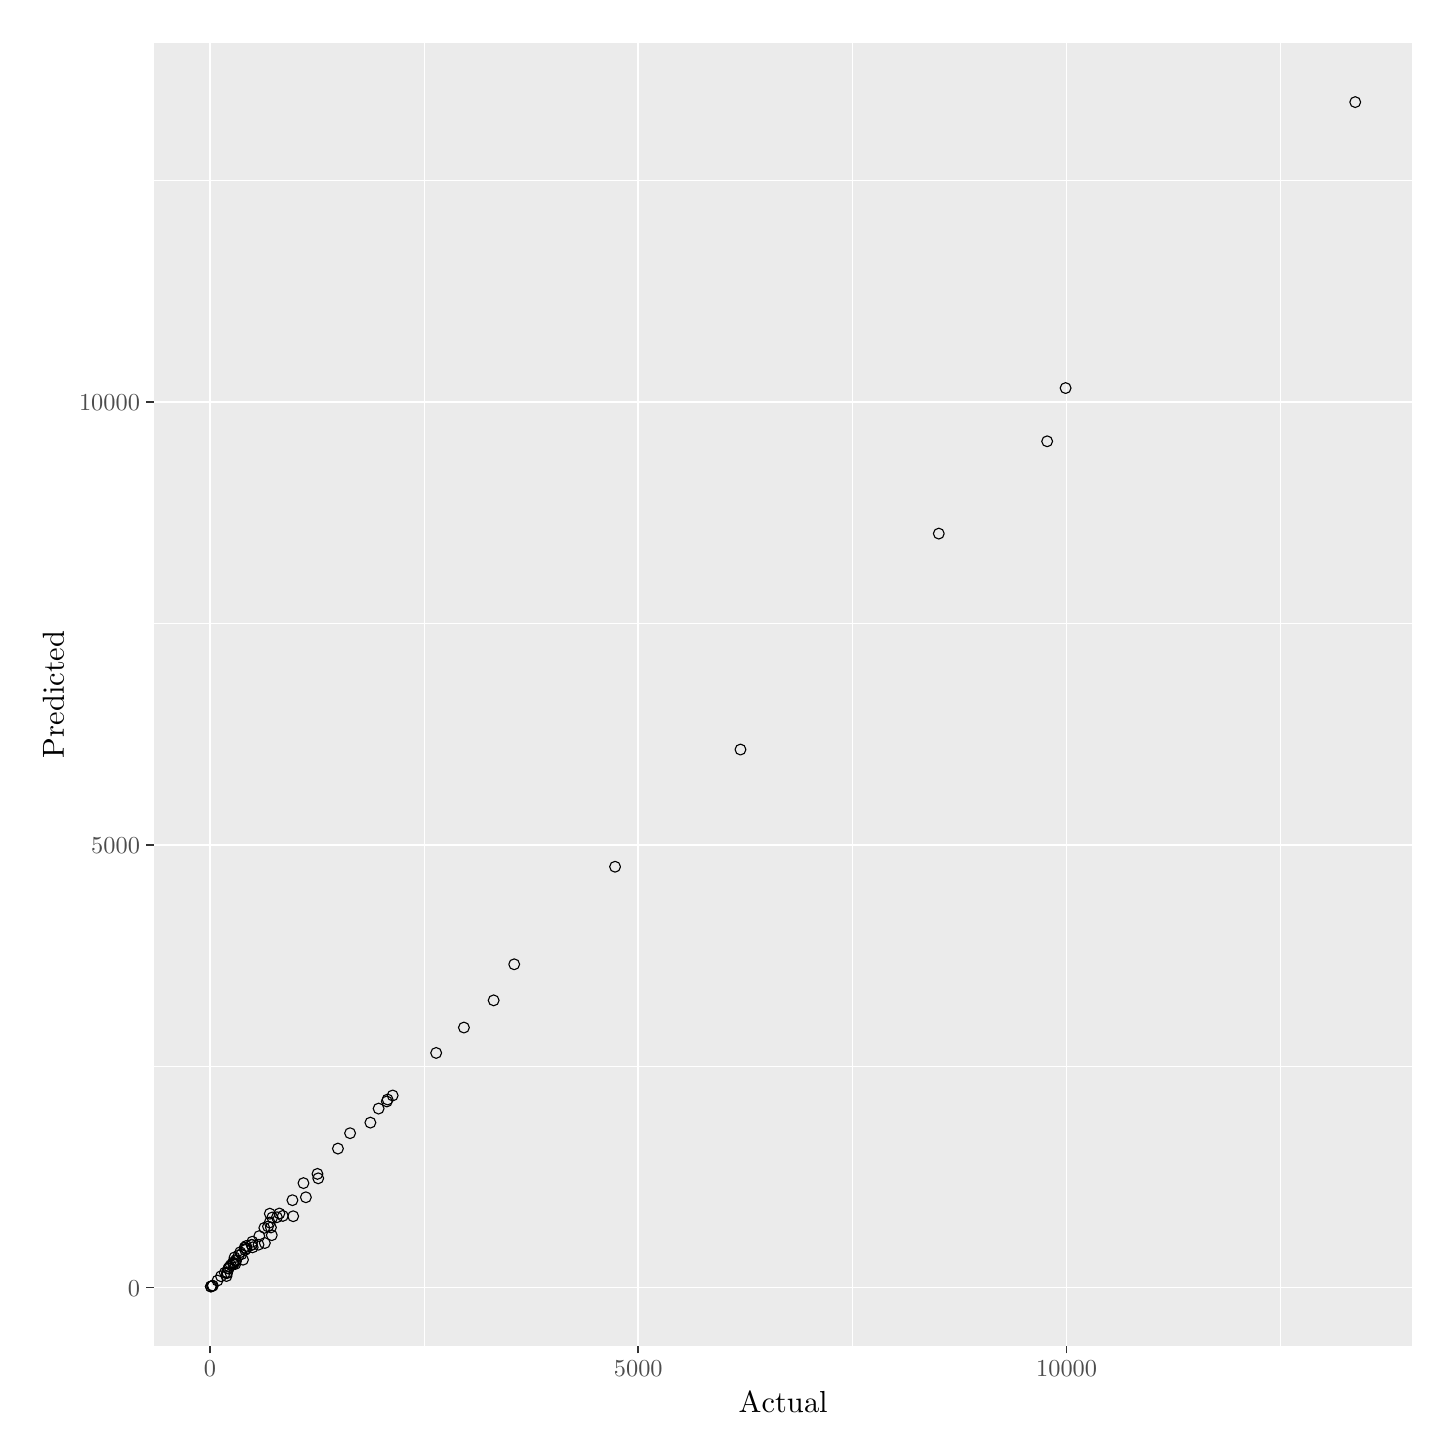
\begin{tikzpicture}[x=1pt,y=1pt]
\definecolor{fillColor}{RGB}{255,255,255}
\path[use as bounding box,fill=fillColor,fill opacity=0.00] (0,0) rectangle (505.89,505.89);
\begin{scope}
\path[clip] (  0.00,  0.00) rectangle (505.89,505.89);
\definecolor{drawColor}{RGB}{255,255,255}
\definecolor{fillColor}{RGB}{255,255,255}

\path[draw=drawColor,line width= 0.6pt,line join=round,line cap=round,fill=fillColor] (  0.00,  0.00) rectangle (505.89,505.89);
\end{scope}
\begin{scope}
\path[clip] ( 45.52, 29.59) rectangle (500.39,500.39);
\definecolor{fillColor}{gray}{0.92}

\path[fill=fillColor] ( 45.52, 29.59) rectangle (500.39,500.39);
\definecolor{drawColor}{RGB}{255,255,255}

\path[draw=drawColor,line width= 0.3pt,line join=round] ( 45.52,130.61) --
	(500.39,130.61);

\path[draw=drawColor,line width= 0.3pt,line join=round] ( 45.52,290.63) --
	(500.39,290.63);

\path[draw=drawColor,line width= 0.3pt,line join=round] ( 45.52,450.66) --
	(500.39,450.66);

\path[draw=drawColor,line width= 0.3pt,line join=round] (143.25, 29.59) --
	(143.25,500.39);

\path[draw=drawColor,line width= 0.3pt,line join=round] (298.03, 29.59) --
	(298.03,500.39);

\path[draw=drawColor,line width= 0.3pt,line join=round] (452.81, 29.59) --
	(452.81,500.39);

\path[draw=drawColor,line width= 0.6pt,line join=round] ( 45.52, 50.60) --
	(500.39, 50.60);

\path[draw=drawColor,line width= 0.6pt,line join=round] ( 45.52,210.62) --
	(500.39,210.62);

\path[draw=drawColor,line width= 0.6pt,line join=round] ( 45.52,370.64) --
	(500.39,370.64);

\path[draw=drawColor,line width= 0.6pt,line join=round] ( 65.86, 29.59) --
	( 65.86,500.39);

\path[draw=drawColor,line width= 0.6pt,line join=round] (220.64, 29.59) --
	(220.64,500.39);

\path[draw=drawColor,line width= 0.6pt,line join=round] (375.42, 29.59) --
	(375.42,500.39);
\definecolor{drawColor}{RGB}{0,0,0}

\path[draw=drawColor,line width= 0.4pt,line join=round,line cap=round] ( 66.20, 50.99) circle (  1.96);

\path[draw=drawColor,line width= 0.4pt,line join=round,line cap=round] ( 66.20, 50.99) circle (  1.96);

\path[draw=drawColor,line width= 0.4pt,line join=round,line cap=round] ( 66.63, 51.22) circle (  1.96);

\path[draw=drawColor,line width= 0.4pt,line join=round,line cap=round] ( 66.91, 51.31) circle (  1.96);

\path[draw=drawColor,line width= 0.4pt,line join=round,line cap=round] ( 68.58, 53.15) circle (  1.96);

\path[draw=drawColor,line width= 0.4pt,line join=round,line cap=round] ( 69.85, 54.72) circle (  1.96);

\path[draw=drawColor,line width= 0.4pt,line join=round,line cap=round] ( 71.24, 55.97) circle (  1.96);

\path[draw=drawColor,line width= 0.4pt,line join=round,line cap=round] ( 71.86, 54.80) circle (  1.96);

\path[draw=drawColor,line width= 0.4pt,line join=round,line cap=round] ( 72.02, 55.82) circle (  1.96);

\path[draw=drawColor,line width= 0.4pt,line join=round,line cap=round] ( 72.08, 56.10) circle (  1.96);

\path[draw=drawColor,line width= 0.4pt,line join=round,line cap=round] ( 72.54, 57.53) circle (  1.96);

\path[draw=drawColor,line width= 0.4pt,line join=round,line cap=round] ( 72.54, 57.53) circle (  1.96);

\path[draw=drawColor,line width= 0.4pt,line join=round,line cap=round] ( 72.91, 58.06) circle (  1.96);

\path[draw=drawColor,line width= 0.4pt,line join=round,line cap=round] ( 73.44, 58.75) circle (  1.96);

\path[draw=drawColor,line width= 0.4pt,line join=round,line cap=round] ( 74.18, 59.70) circle (  1.96);

\path[draw=drawColor,line width= 0.4pt,line join=round,line cap=round] ( 74.25, 59.24) circle (  1.96);

\path[draw=drawColor,line width= 0.4pt,line join=round,line cap=round] ( 74.46, 59.24) circle (  1.96);

\path[draw=drawColor,line width= 0.4pt,line join=round,line cap=round] ( 74.77, 61.55) circle (  1.96);

\path[draw=drawColor,line width= 0.4pt,line join=round,line cap=round] ( 75.05, 59.15) circle (  1.96);

\path[draw=drawColor,line width= 0.4pt,line join=round,line cap=round] ( 75.27, 60.63) circle (  1.96);

\path[draw=drawColor,line width= 0.4pt,line join=round,line cap=round] ( 75.30, 60.28) circle (  1.96);

\path[draw=drawColor,line width= 0.4pt,line join=round,line cap=round] ( 76.20, 62.20) circle (  1.96);

\path[draw=drawColor,line width= 0.4pt,line join=round,line cap=round] ( 76.81, 63.40) circle (  1.96);

\path[draw=drawColor,line width= 0.4pt,line join=round,line cap=round] ( 77.25, 62.70) circle (  1.96);

\path[draw=drawColor,line width= 0.4pt,line join=round,line cap=round] ( 77.81, 60.69) circle (  1.96);

\path[draw=drawColor,line width= 0.4pt,line join=round,line cap=round] ( 78.39, 65.06) circle (  1.96);

\path[draw=drawColor,line width= 0.4pt,line join=round,line cap=round] ( 78.58, 64.23) circle (  1.96);

\path[draw=drawColor,line width= 0.4pt,line join=round,line cap=round] ( 78.95, 65.65) circle (  1.96);

\path[draw=drawColor,line width= 0.4pt,line join=round,line cap=round] ( 79.01, 64.72) circle (  1.96);

\path[draw=drawColor,line width= 0.4pt,line join=round,line cap=round] ( 80.96, 66.06) circle (  1.96);

\path[draw=drawColor,line width= 0.4pt,line join=round,line cap=round] ( 80.96, 66.06) circle (  1.96);

\path[draw=drawColor,line width= 0.4pt,line join=round,line cap=round] ( 81.18, 67.20) circle (  1.96);

\path[draw=drawColor,line width= 0.4pt,line join=round,line cap=round] ( 81.30, 65.17) circle (  1.96);

\path[draw=drawColor,line width= 0.4pt,line join=round,line cap=round] ( 83.41, 66.12) circle (  1.96);

\path[draw=drawColor,line width= 0.4pt,line join=round,line cap=round] ( 83.69, 69.24) circle (  1.96);

\path[draw=drawColor,line width= 0.4pt,line join=round,line cap=round] ( 85.51, 72.20) circle (  1.96);

\path[draw=drawColor,line width= 0.4pt,line join=round,line cap=round] ( 85.70, 66.72) circle (  1.96);

\path[draw=drawColor,line width= 0.4pt,line join=round,line cap=round] ( 86.84, 72.70) circle (  1.96);

\path[draw=drawColor,line width= 0.4pt,line join=round,line cap=round] ( 87.43, 74.12) circle (  1.96);

\path[draw=drawColor,line width= 0.4pt,line join=round,line cap=round] ( 87.49, 77.33) circle (  1.96);

\path[draw=drawColor,line width= 0.4pt,line join=round,line cap=round] ( 87.90, 72.34) circle (  1.96);

\path[draw=drawColor,line width= 0.4pt,line join=round,line cap=round] ( 88.21, 69.55) circle (  1.96);

\path[draw=drawColor,line width= 0.4pt,line join=round,line cap=round] ( 88.39, 75.96) circle (  1.96);

\path[draw=drawColor,line width= 0.4pt,line join=round,line cap=round] ( 90.06, 76.03) circle (  1.96);

\path[draw=drawColor,line width= 0.4pt,line join=round,line cap=round] ( 90.96, 77.39) circle (  1.96);

\path[draw=drawColor,line width= 0.4pt,line join=round,line cap=round] ( 92.20, 76.52) circle (  1.96);

\path[draw=drawColor,line width= 0.4pt,line join=round,line cap=round] ( 95.67, 82.20) circle (  1.96);

\path[draw=drawColor,line width= 0.4pt,line join=round,line cap=round] ( 95.95, 76.40) circle (  1.96);

\path[draw=drawColor,line width= 0.4pt,line join=round,line cap=round] ( 99.66, 88.37) circle (  1.96);

\path[draw=drawColor,line width= 0.4pt,line join=round,line cap=round] (100.53, 83.25) circle (  1.96);

\path[draw=drawColor,line width= 0.4pt,line join=round,line cap=round] (104.71, 91.70) circle (  1.96);

\path[draw=drawColor,line width= 0.4pt,line join=round,line cap=round] (104.99, 90.10) circle (  1.96);

\path[draw=drawColor,line width= 0.4pt,line join=round,line cap=round] (112.11,100.85) circle (  1.96);

\path[draw=drawColor,line width= 0.4pt,line join=round,line cap=round] (116.50,106.41) circle (  1.96);

\path[draw=drawColor,line width= 0.4pt,line join=round,line cap=round] (123.84,110.23) circle (  1.96);

\path[draw=drawColor,line width= 0.4pt,line join=round,line cap=round] (126.81,115.30) circle (  1.96);

\path[draw=drawColor,line width= 0.4pt,line join=round,line cap=round] (129.78,117.88) circle (  1.96);

\path[draw=drawColor,line width= 0.4pt,line join=round,line cap=round] (130.06,118.58) circle (  1.96);

\path[draw=drawColor,line width= 0.4pt,line join=round,line cap=round] (131.89,120.03) circle (  1.96);

\path[draw=drawColor,line width= 0.4pt,line join=round,line cap=round] (147.61,135.41) circle (  1.96);

\path[draw=drawColor,line width= 0.4pt,line join=round,line cap=round] (157.64,144.58) circle (  1.96);

\path[draw=drawColor,line width= 0.4pt,line join=round,line cap=round] (168.38,154.41) circle (  1.96);

\path[draw=drawColor,line width= 0.4pt,line join=round,line cap=round] (175.81,167.44) circle (  1.96);

\path[draw=drawColor,line width= 0.4pt,line join=round,line cap=round] (212.25,202.69) circle (  1.96);

\path[draw=drawColor,line width= 0.4pt,line join=round,line cap=round] (257.57,245.04) circle (  1.96);

\path[draw=drawColor,line width= 0.4pt,line join=round,line cap=round] (329.23,323.07) circle (  1.96);

\path[draw=drawColor,line width= 0.4pt,line join=round,line cap=round] (368.39,356.42) circle (  1.96);

\path[draw=drawColor,line width= 0.4pt,line join=round,line cap=round] (375.05,375.66) circle (  1.96);

\path[draw=drawColor,line width= 0.4pt,line join=round,line cap=round] (479.71,478.99) circle (  1.96);
\end{scope}
\begin{scope}
\path[clip] (  0.00,  0.00) rectangle (505.89,505.89);
\definecolor{drawColor}{gray}{0.30}

\node[text=drawColor,anchor=base east,inner sep=0pt, outer sep=0pt, scale=  0.88] at ( 40.57, 47.57) {0};

\node[text=drawColor,anchor=base east,inner sep=0pt, outer sep=0pt, scale=  0.88] at ( 40.57,207.59) {5000};

\node[text=drawColor,anchor=base east,inner sep=0pt, outer sep=0pt, scale=  0.88] at ( 40.57,367.61) {10000};
\end{scope}
\begin{scope}
\path[clip] (  0.00,  0.00) rectangle (505.89,505.89);
\definecolor{drawColor}{gray}{0.20}

\path[draw=drawColor,line width= 0.6pt,line join=round] ( 42.77, 50.60) --
	( 45.52, 50.60);

\path[draw=drawColor,line width= 0.6pt,line join=round] ( 42.77,210.62) --
	( 45.52,210.62);

\path[draw=drawColor,line width= 0.6pt,line join=round] ( 42.77,370.64) --
	( 45.52,370.64);
\end{scope}
\begin{scope}
\path[clip] (  0.00,  0.00) rectangle (505.89,505.89);
\definecolor{drawColor}{gray}{0.20}

\path[draw=drawColor,line width= 0.6pt,line join=round] ( 65.86, 26.84) --
	( 65.86, 29.59);

\path[draw=drawColor,line width= 0.6pt,line join=round] (220.64, 26.84) --
	(220.64, 29.59);

\path[draw=drawColor,line width= 0.6pt,line join=round] (375.42, 26.84) --
	(375.42, 29.59);
\end{scope}
\begin{scope}
\path[clip] (  0.00,  0.00) rectangle (505.89,505.89);
\definecolor{drawColor}{gray}{0.30}

\node[text=drawColor,anchor=base,inner sep=0pt, outer sep=0pt, scale=  0.88] at ( 65.86, 18.58) {0};

\node[text=drawColor,anchor=base,inner sep=0pt, outer sep=0pt, scale=  0.88] at (220.64, 18.58) {5000};

\node[text=drawColor,anchor=base,inner sep=0pt, outer sep=0pt, scale=  0.88] at (375.42, 18.58) {10000};
\end{scope}
\begin{scope}
\path[clip] (  0.00,  0.00) rectangle (505.89,505.89);
\definecolor{drawColor}{RGB}{0,0,0}

\node[text=drawColor,anchor=base,inner sep=0pt, outer sep=0pt, scale=  1.10] at (272.96,  5.50) {Actual};
\end{scope}
\begin{scope}
\path[clip] (  0.00,  0.00) rectangle (505.89,505.89);
\definecolor{drawColor}{RGB}{0,0,0}

\node[text=drawColor,rotate= 90.00,anchor=base,inner sep=0pt, outer sep=0pt, scale=  1.10] at ( 13.08,264.99) {Predicted};
\end{scope}
\end{tikzpicture}
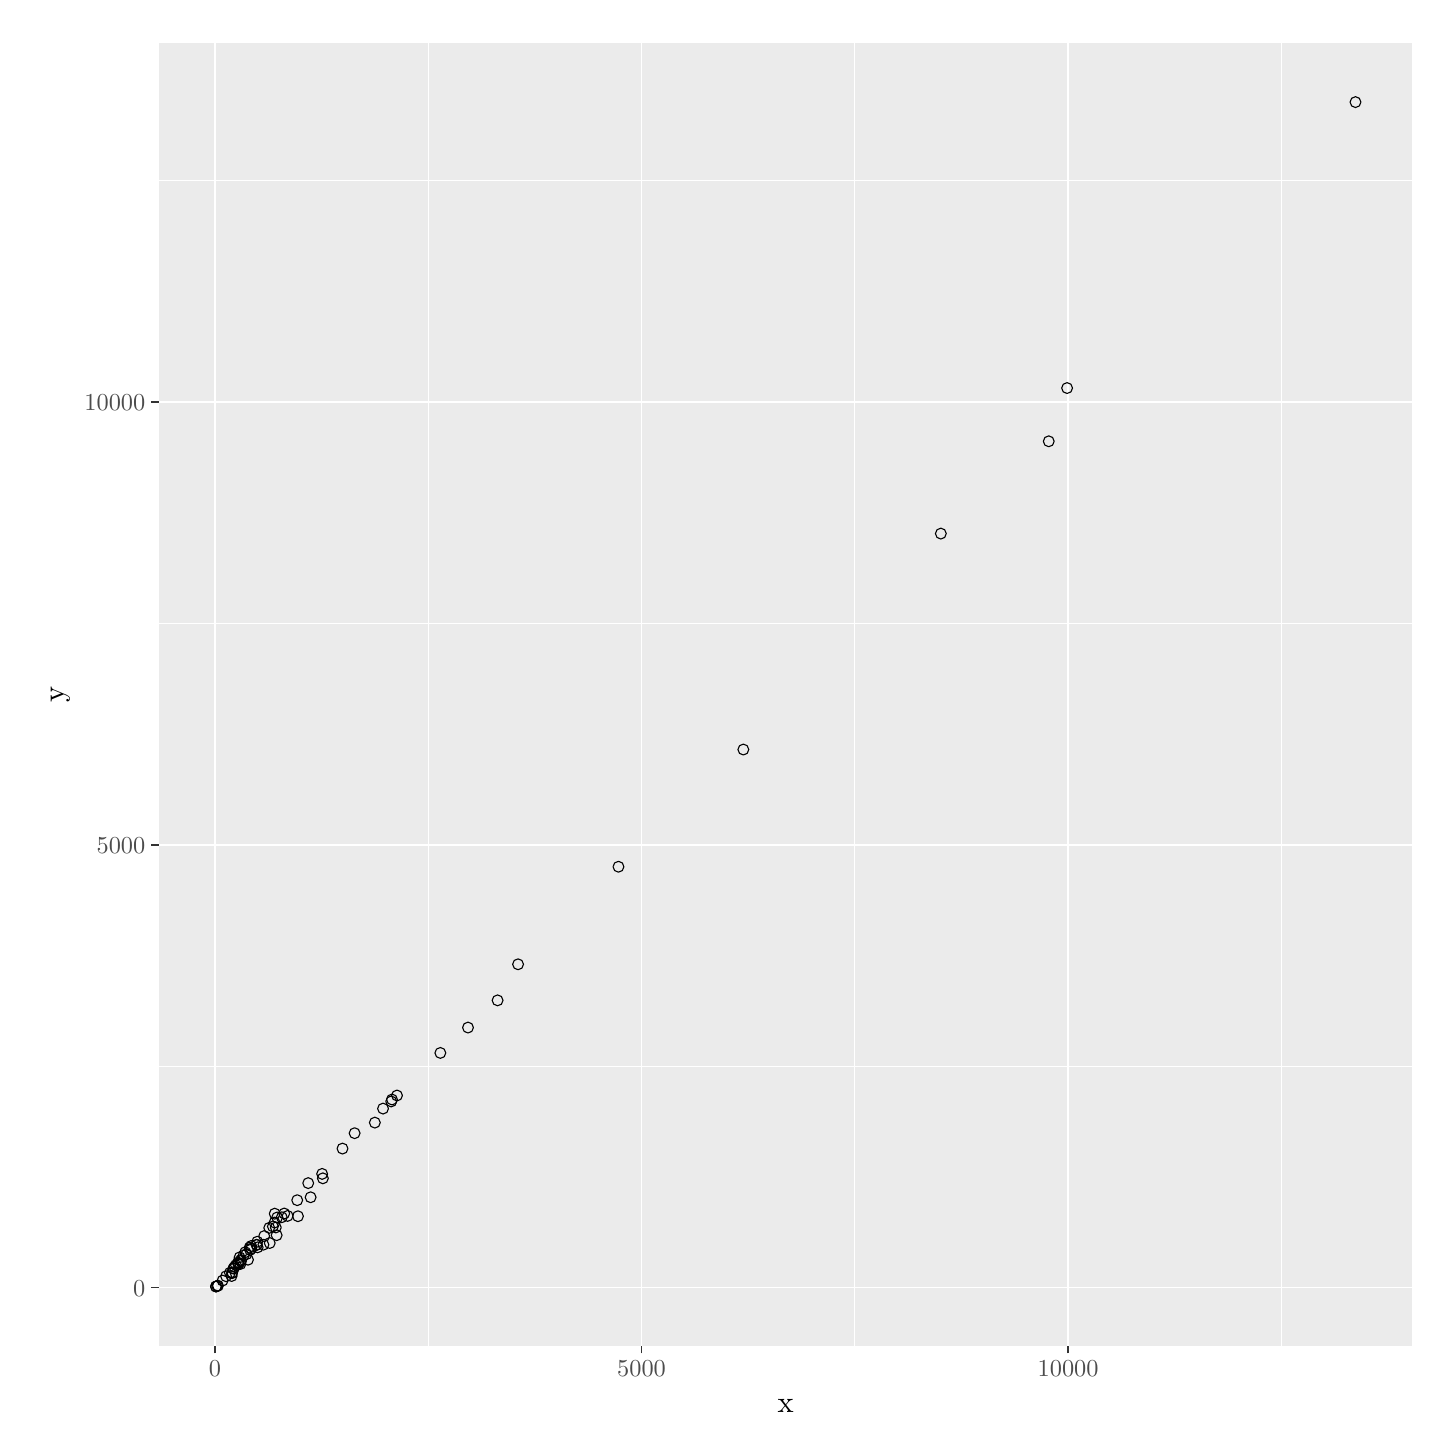
\begin{tikzpicture}[x=1pt,y=1pt]
\definecolor{fillColor}{RGB}{255,255,255}
\path[use as bounding box,fill=fillColor,fill opacity=0.00] (0,0) rectangle (505.89,505.89);
\begin{scope}
\path[clip] (  0.00,  0.00) rectangle (505.89,505.89);
\definecolor{drawColor}{RGB}{255,255,255}
\definecolor{fillColor}{RGB}{255,255,255}

\path[draw=drawColor,line width= 0.6pt,line join=round,line cap=round,fill=fillColor] (  0.00,  0.00) rectangle (505.89,505.89);
\end{scope}
\begin{scope}
\path[clip] ( 47.46, 29.59) rectangle (500.39,500.39);
\definecolor{fillColor}{gray}{0.92}

\path[fill=fillColor] ( 47.46, 29.59) rectangle (500.39,500.39);
\definecolor{drawColor}{RGB}{255,255,255}

\path[draw=drawColor,line width= 0.3pt,line join=round] ( 47.46,130.61) --
	(500.39,130.61);

\path[draw=drawColor,line width= 0.3pt,line join=round] ( 47.46,290.63) --
	(500.39,290.63);

\path[draw=drawColor,line width= 0.3pt,line join=round] ( 47.46,450.66) --
	(500.39,450.66);

\path[draw=drawColor,line width= 0.3pt,line join=round] (144.77, 29.59) --
	(144.77,500.39);

\path[draw=drawColor,line width= 0.3pt,line join=round] (298.89, 29.59) --
	(298.89,500.39);

\path[draw=drawColor,line width= 0.3pt,line join=round] (453.02, 29.59) --
	(453.02,500.39);

\path[draw=drawColor,line width= 0.6pt,line join=round] ( 47.46, 50.60) --
	(500.39, 50.60);

\path[draw=drawColor,line width= 0.6pt,line join=round] ( 47.46,210.62) --
	(500.39,210.62);

\path[draw=drawColor,line width= 0.6pt,line join=round] ( 47.46,370.64) --
	(500.39,370.64);

\path[draw=drawColor,line width= 0.6pt,line join=round] ( 67.71, 29.59) --
	( 67.71,500.39);

\path[draw=drawColor,line width= 0.6pt,line join=round] (221.83, 29.59) --
	(221.83,500.39);

\path[draw=drawColor,line width= 0.6pt,line join=round] (375.96, 29.59) --
	(375.96,500.39);
\definecolor{drawColor}{RGB}{0,0,0}

\path[draw=drawColor,line width= 0.4pt,line join=round,line cap=round] ( 68.05, 50.99) circle (  1.96);

\path[draw=drawColor,line width= 0.4pt,line join=round,line cap=round] ( 68.05, 50.99) circle (  1.96);

\path[draw=drawColor,line width= 0.4pt,line join=round,line cap=round] ( 68.48, 51.22) circle (  1.96);

\path[draw=drawColor,line width= 0.4pt,line join=round,line cap=round] ( 68.76, 51.31) circle (  1.96);

\path[draw=drawColor,line width= 0.4pt,line join=round,line cap=round] ( 70.43, 53.15) circle (  1.96);

\path[draw=drawColor,line width= 0.4pt,line join=round,line cap=round] ( 71.69, 54.72) circle (  1.96);

\path[draw=drawColor,line width= 0.4pt,line join=round,line cap=round] ( 73.08, 55.97) circle (  1.96);

\path[draw=drawColor,line width= 0.4pt,line join=round,line cap=round] ( 73.69, 54.80) circle (  1.96);

\path[draw=drawColor,line width= 0.4pt,line join=round,line cap=round] ( 73.85, 55.82) circle (  1.96);

\path[draw=drawColor,line width= 0.4pt,line join=round,line cap=round] ( 73.91, 56.10) circle (  1.96);

\path[draw=drawColor,line width= 0.4pt,line join=round,line cap=round] ( 74.37, 57.53) circle (  1.96);

\path[draw=drawColor,line width= 0.4pt,line join=round,line cap=round] ( 74.37, 57.53) circle (  1.96);

\path[draw=drawColor,line width= 0.4pt,line join=round,line cap=round] ( 74.74, 58.06) circle (  1.96);

\path[draw=drawColor,line width= 0.4pt,line join=round,line cap=round] ( 75.27, 58.75) circle (  1.96);

\path[draw=drawColor,line width= 0.4pt,line join=round,line cap=round] ( 76.00, 59.70) circle (  1.96);

\path[draw=drawColor,line width= 0.4pt,line join=round,line cap=round] ( 76.07, 59.24) circle (  1.96);

\path[draw=drawColor,line width= 0.4pt,line join=round,line cap=round] ( 76.28, 59.24) circle (  1.96);

\path[draw=drawColor,line width= 0.4pt,line join=round,line cap=round] ( 76.59, 61.55) circle (  1.96);

\path[draw=drawColor,line width= 0.4pt,line join=round,line cap=round] ( 76.87, 59.15) circle (  1.96);

\path[draw=drawColor,line width= 0.4pt,line join=round,line cap=round] ( 77.08, 60.63) circle (  1.96);

\path[draw=drawColor,line width= 0.4pt,line join=round,line cap=round] ( 77.11, 60.28) circle (  1.96);

\path[draw=drawColor,line width= 0.4pt,line join=round,line cap=round] ( 78.01, 62.20) circle (  1.96);

\path[draw=drawColor,line width= 0.4pt,line join=round,line cap=round] ( 78.62, 63.40) circle (  1.96);

\path[draw=drawColor,line width= 0.4pt,line join=round,line cap=round] ( 79.06, 62.70) circle (  1.96);

\path[draw=drawColor,line width= 0.4pt,line join=round,line cap=round] ( 79.61, 60.69) circle (  1.96);

\path[draw=drawColor,line width= 0.4pt,line join=round,line cap=round] ( 80.20, 65.06) circle (  1.96);

\path[draw=drawColor,line width= 0.4pt,line join=round,line cap=round] ( 80.38, 64.23) circle (  1.96);

\path[draw=drawColor,line width= 0.4pt,line join=round,line cap=round] ( 80.75, 65.65) circle (  1.96);

\path[draw=drawColor,line width= 0.4pt,line join=round,line cap=round] ( 80.81, 64.72) circle (  1.96);

\path[draw=drawColor,line width= 0.4pt,line join=round,line cap=round] ( 82.76, 66.06) circle (  1.96);

\path[draw=drawColor,line width= 0.4pt,line join=round,line cap=round] ( 82.76, 66.06) circle (  1.96);

\path[draw=drawColor,line width= 0.4pt,line join=round,line cap=round] ( 82.97, 67.20) circle (  1.96);

\path[draw=drawColor,line width= 0.4pt,line join=round,line cap=round] ( 83.09, 65.17) circle (  1.96);

\path[draw=drawColor,line width= 0.4pt,line join=round,line cap=round] ( 85.19, 66.12) circle (  1.96);

\path[draw=drawColor,line width= 0.4pt,line join=round,line cap=round] ( 85.47, 69.24) circle (  1.96);

\path[draw=drawColor,line width= 0.4pt,line join=round,line cap=round] ( 87.29, 72.20) circle (  1.96);

\path[draw=drawColor,line width= 0.4pt,line join=round,line cap=round] ( 87.47, 66.72) circle (  1.96);

\path[draw=drawColor,line width= 0.4pt,line join=round,line cap=round] ( 88.61, 72.70) circle (  1.96);

\path[draw=drawColor,line width= 0.4pt,line join=round,line cap=round] ( 89.20, 74.12) circle (  1.96);

\path[draw=drawColor,line width= 0.4pt,line join=round,line cap=round] ( 89.26, 77.33) circle (  1.96);

\path[draw=drawColor,line width= 0.4pt,line join=round,line cap=round] ( 89.66, 72.34) circle (  1.96);

\path[draw=drawColor,line width= 0.4pt,line join=round,line cap=round] ( 89.97, 69.55) circle (  1.96);

\path[draw=drawColor,line width= 0.4pt,line join=round,line cap=round] ( 90.15, 75.96) circle (  1.96);

\path[draw=drawColor,line width= 0.4pt,line join=round,line cap=round] ( 91.82, 76.03) circle (  1.96);

\path[draw=drawColor,line width= 0.4pt,line join=round,line cap=round] ( 92.71, 77.39) circle (  1.96);

\path[draw=drawColor,line width= 0.4pt,line join=round,line cap=round] ( 93.94, 76.52) circle (  1.96);

\path[draw=drawColor,line width= 0.4pt,line join=round,line cap=round] ( 97.40, 82.20) circle (  1.96);

\path[draw=drawColor,line width= 0.4pt,line join=round,line cap=round] ( 97.67, 76.40) circle (  1.96);

\path[draw=drawColor,line width= 0.4pt,line join=round,line cap=round] (101.37, 88.37) circle (  1.96);

\path[draw=drawColor,line width= 0.4pt,line join=round,line cap=round] (102.24, 83.25) circle (  1.96);

\path[draw=drawColor,line width= 0.4pt,line join=round,line cap=round] (106.40, 91.70) circle (  1.96);

\path[draw=drawColor,line width= 0.4pt,line join=round,line cap=round] (106.67, 90.10) circle (  1.96);

\path[draw=drawColor,line width= 0.4pt,line join=round,line cap=round] (113.76,100.85) circle (  1.96);

\path[draw=drawColor,line width= 0.4pt,line join=round,line cap=round] (118.14,106.41) circle (  1.96);

\path[draw=drawColor,line width= 0.4pt,line join=round,line cap=round] (125.45,110.23) circle (  1.96);

\path[draw=drawColor,line width= 0.4pt,line join=round,line cap=round] (128.41,115.30) circle (  1.96);

\path[draw=drawColor,line width= 0.4pt,line join=round,line cap=round] (131.37,117.88) circle (  1.96);

\path[draw=drawColor,line width= 0.4pt,line join=round,line cap=round] (131.64,118.58) circle (  1.96);

\path[draw=drawColor,line width= 0.4pt,line join=round,line cap=round] (133.46,120.03) circle (  1.96);

\path[draw=drawColor,line width= 0.4pt,line join=round,line cap=round] (149.12,135.41) circle (  1.96);

\path[draw=drawColor,line width= 0.4pt,line join=round,line cap=round] (159.11,144.58) circle (  1.96);

\path[draw=drawColor,line width= 0.4pt,line join=round,line cap=round] (169.80,154.41) circle (  1.96);

\path[draw=drawColor,line width= 0.4pt,line join=round,line cap=round] (177.20,167.44) circle (  1.96);

\path[draw=drawColor,line width= 0.4pt,line join=round,line cap=round] (213.48,202.69) circle (  1.96);

\path[draw=drawColor,line width= 0.4pt,line join=round,line cap=round] (258.61,245.04) circle (  1.96);

\path[draw=drawColor,line width= 0.4pt,line join=round,line cap=round] (329.97,323.07) circle (  1.96);

\path[draw=drawColor,line width= 0.4pt,line join=round,line cap=round] (368.96,356.42) circle (  1.96);

\path[draw=drawColor,line width= 0.4pt,line join=round,line cap=round] (375.59,375.66) circle (  1.96);

\path[draw=drawColor,line width= 0.4pt,line join=round,line cap=round] (479.80,478.99) circle (  1.96);
\end{scope}
\begin{scope}
\path[clip] (  0.00,  0.00) rectangle (505.89,505.89);
\definecolor{drawColor}{gray}{0.30}

\node[text=drawColor,anchor=base east,inner sep=0pt, outer sep=0pt, scale=  0.88] at ( 42.51, 47.57) {0};

\node[text=drawColor,anchor=base east,inner sep=0pt, outer sep=0pt, scale=  0.88] at ( 42.51,207.59) {5000};

\node[text=drawColor,anchor=base east,inner sep=0pt, outer sep=0pt, scale=  0.88] at ( 42.51,367.61) {10000};
\end{scope}
\begin{scope}
\path[clip] (  0.00,  0.00) rectangle (505.89,505.89);
\definecolor{drawColor}{gray}{0.20}

\path[draw=drawColor,line width= 0.6pt,line join=round] ( 44.71, 50.60) --
	( 47.46, 50.60);

\path[draw=drawColor,line width= 0.6pt,line join=round] ( 44.71,210.62) --
	( 47.46,210.62);

\path[draw=drawColor,line width= 0.6pt,line join=round] ( 44.71,370.64) --
	( 47.46,370.64);
\end{scope}
\begin{scope}
\path[clip] (  0.00,  0.00) rectangle (505.89,505.89);
\definecolor{drawColor}{gray}{0.20}

\path[draw=drawColor,line width= 0.6pt,line join=round] ( 67.71, 26.84) --
	( 67.71, 29.59);

\path[draw=drawColor,line width= 0.6pt,line join=round] (221.83, 26.84) --
	(221.83, 29.59);

\path[draw=drawColor,line width= 0.6pt,line join=round] (375.96, 26.84) --
	(375.96, 29.59);
\end{scope}
\begin{scope}
\path[clip] (  0.00,  0.00) rectangle (505.89,505.89);
\definecolor{drawColor}{gray}{0.30}

\node[text=drawColor,anchor=base,inner sep=0pt, outer sep=0pt, scale=  0.88] at ( 67.71, 18.58) {0};

\node[text=drawColor,anchor=base,inner sep=0pt, outer sep=0pt, scale=  0.88] at (221.83, 18.58) {5000};

\node[text=drawColor,anchor=base,inner sep=0pt, outer sep=0pt, scale=  0.88] at (375.96, 18.58) {10000};
\end{scope}
\begin{scope}
\path[clip] (  0.00,  0.00) rectangle (505.89,505.89);
\definecolor{drawColor}{RGB}{0,0,0}

\node[text=drawColor,anchor=base,inner sep=0pt, outer sep=0pt, scale=  1.10] at (273.93,  5.50) {x};
\end{scope}
\begin{scope}
\path[clip] (  0.00,  0.00) rectangle (505.89,505.89);
\definecolor{drawColor}{RGB}{0,0,0}

\node[text=drawColor,rotate= 90.00,anchor=base,inner sep=0pt, outer sep=0pt, scale=  1.10] at ( 13.08,264.99) {y};
\end{scope}
\end{tikzpicture}
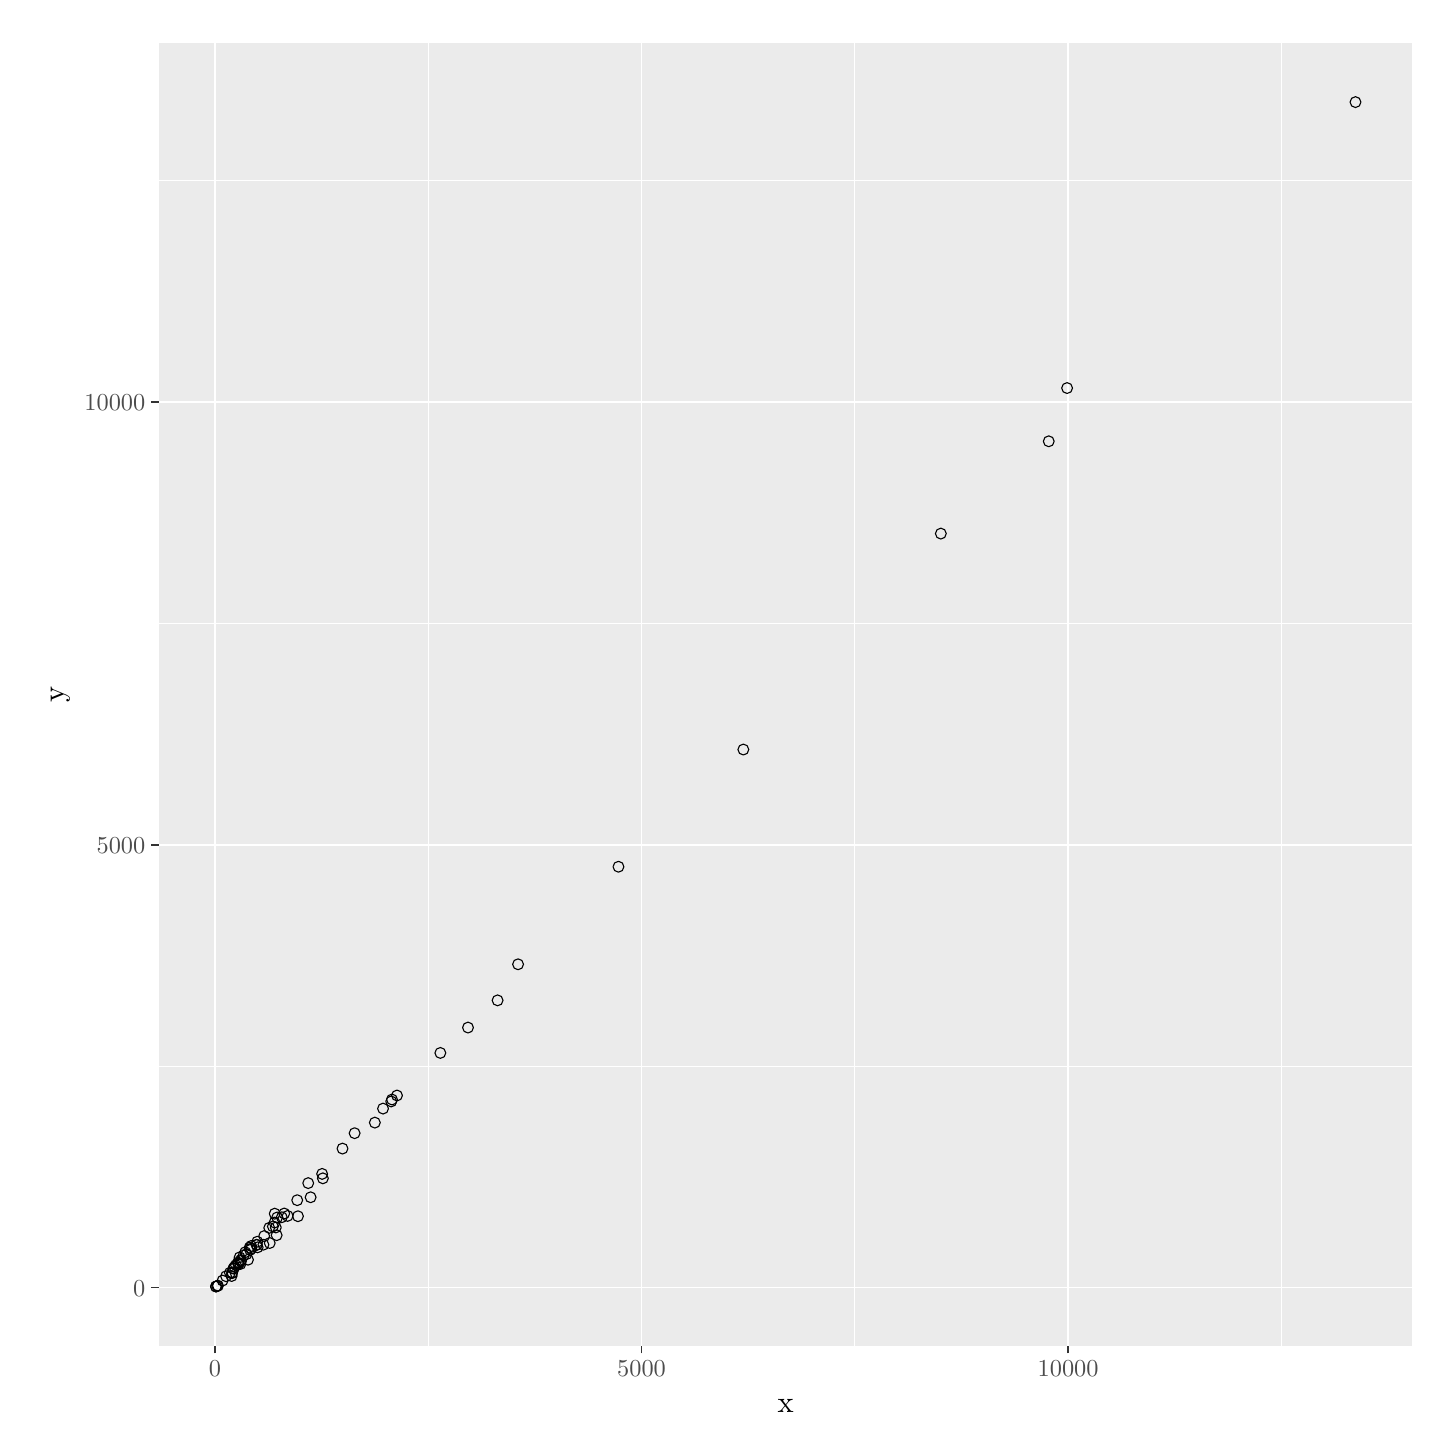
\begin{tikzpicture}[x=1pt,y=1pt]
\definecolor{fillColor}{RGB}{255,255,255}
\path[use as bounding box,fill=fillColor,fill opacity=0.00] (0,0) rectangle (505.89,505.89);
\begin{scope}
\path[clip] (  0.00,  0.00) rectangle (505.89,505.89);
\definecolor{drawColor}{RGB}{255,255,255}
\definecolor{fillColor}{RGB}{255,255,255}

\path[draw=drawColor,line width= 0.6pt,line join=round,line cap=round,fill=fillColor] (  0.00,  0.00) rectangle (505.89,505.89);
\end{scope}
\begin{scope}
\path[clip] ( 47.46, 29.59) rectangle (500.39,500.39);
\definecolor{fillColor}{gray}{0.92}

\path[fill=fillColor] ( 47.46, 29.59) rectangle (500.39,500.39);
\definecolor{drawColor}{RGB}{255,255,255}

\path[draw=drawColor,line width= 0.3pt,line join=round] ( 47.46,130.61) --
	(500.39,130.61);

\path[draw=drawColor,line width= 0.3pt,line join=round] ( 47.46,290.63) --
	(500.39,290.63);

\path[draw=drawColor,line width= 0.3pt,line join=round] ( 47.46,450.66) --
	(500.39,450.66);

\path[draw=drawColor,line width= 0.3pt,line join=round] (144.77, 29.59) --
	(144.77,500.39);

\path[draw=drawColor,line width= 0.3pt,line join=round] (298.89, 29.59) --
	(298.89,500.39);

\path[draw=drawColor,line width= 0.3pt,line join=round] (453.02, 29.59) --
	(453.02,500.39);

\path[draw=drawColor,line width= 0.6pt,line join=round] ( 47.46, 50.60) --
	(500.39, 50.60);

\path[draw=drawColor,line width= 0.6pt,line join=round] ( 47.46,210.62) --
	(500.39,210.62);

\path[draw=drawColor,line width= 0.6pt,line join=round] ( 47.46,370.64) --
	(500.39,370.64);

\path[draw=drawColor,line width= 0.6pt,line join=round] ( 67.71, 29.59) --
	( 67.71,500.39);

\path[draw=drawColor,line width= 0.6pt,line join=round] (221.83, 29.59) --
	(221.83,500.39);

\path[draw=drawColor,line width= 0.6pt,line join=round] (375.96, 29.59) --
	(375.96,500.39);
\definecolor{drawColor}{RGB}{0,0,0}

\path[draw=drawColor,line width= 0.4pt,line join=round,line cap=round] ( 68.05, 50.99) circle (  1.96);

\path[draw=drawColor,line width= 0.4pt,line join=round,line cap=round] ( 68.05, 50.99) circle (  1.96);

\path[draw=drawColor,line width= 0.4pt,line join=round,line cap=round] ( 68.48, 51.22) circle (  1.96);

\path[draw=drawColor,line width= 0.4pt,line join=round,line cap=round] ( 68.76, 51.31) circle (  1.96);

\path[draw=drawColor,line width= 0.4pt,line join=round,line cap=round] ( 70.43, 53.15) circle (  1.96);

\path[draw=drawColor,line width= 0.4pt,line join=round,line cap=round] ( 71.69, 54.72) circle (  1.96);

\path[draw=drawColor,line width= 0.4pt,line join=round,line cap=round] ( 73.08, 55.97) circle (  1.96);

\path[draw=drawColor,line width= 0.4pt,line join=round,line cap=round] ( 73.69, 54.80) circle (  1.96);

\path[draw=drawColor,line width= 0.4pt,line join=round,line cap=round] ( 73.85, 55.82) circle (  1.96);

\path[draw=drawColor,line width= 0.4pt,line join=round,line cap=round] ( 73.91, 56.10) circle (  1.96);

\path[draw=drawColor,line width= 0.4pt,line join=round,line cap=round] ( 74.37, 57.53) circle (  1.96);

\path[draw=drawColor,line width= 0.4pt,line join=round,line cap=round] ( 74.37, 57.53) circle (  1.96);

\path[draw=drawColor,line width= 0.4pt,line join=round,line cap=round] ( 74.74, 58.06) circle (  1.96);

\path[draw=drawColor,line width= 0.4pt,line join=round,line cap=round] ( 75.27, 58.75) circle (  1.96);

\path[draw=drawColor,line width= 0.4pt,line join=round,line cap=round] ( 76.00, 59.70) circle (  1.96);

\path[draw=drawColor,line width= 0.4pt,line join=round,line cap=round] ( 76.07, 59.24) circle (  1.96);

\path[draw=drawColor,line width= 0.4pt,line join=round,line cap=round] ( 76.28, 59.24) circle (  1.96);

\path[draw=drawColor,line width= 0.4pt,line join=round,line cap=round] ( 76.59, 61.55) circle (  1.96);

\path[draw=drawColor,line width= 0.4pt,line join=round,line cap=round] ( 76.87, 59.15) circle (  1.96);

\path[draw=drawColor,line width= 0.4pt,line join=round,line cap=round] ( 77.08, 60.63) circle (  1.96);

\path[draw=drawColor,line width= 0.4pt,line join=round,line cap=round] ( 77.11, 60.28) circle (  1.96);

\path[draw=drawColor,line width= 0.4pt,line join=round,line cap=round] ( 78.01, 62.20) circle (  1.96);

\path[draw=drawColor,line width= 0.4pt,line join=round,line cap=round] ( 78.62, 63.40) circle (  1.96);

\path[draw=drawColor,line width= 0.4pt,line join=round,line cap=round] ( 79.06, 62.70) circle (  1.96);

\path[draw=drawColor,line width= 0.4pt,line join=round,line cap=round] ( 79.61, 60.69) circle (  1.96);

\path[draw=drawColor,line width= 0.4pt,line join=round,line cap=round] ( 80.20, 65.06) circle (  1.96);

\path[draw=drawColor,line width= 0.4pt,line join=round,line cap=round] ( 80.38, 64.23) circle (  1.96);

\path[draw=drawColor,line width= 0.4pt,line join=round,line cap=round] ( 80.75, 65.65) circle (  1.96);

\path[draw=drawColor,line width= 0.4pt,line join=round,line cap=round] ( 80.81, 64.72) circle (  1.96);

\path[draw=drawColor,line width= 0.4pt,line join=round,line cap=round] ( 82.76, 66.06) circle (  1.96);

\path[draw=drawColor,line width= 0.4pt,line join=round,line cap=round] ( 82.76, 66.06) circle (  1.96);

\path[draw=drawColor,line width= 0.4pt,line join=round,line cap=round] ( 82.97, 67.20) circle (  1.96);

\path[draw=drawColor,line width= 0.4pt,line join=round,line cap=round] ( 83.09, 65.17) circle (  1.96);

\path[draw=drawColor,line width= 0.4pt,line join=round,line cap=round] ( 85.19, 66.12) circle (  1.96);

\path[draw=drawColor,line width= 0.4pt,line join=round,line cap=round] ( 85.47, 69.24) circle (  1.96);

\path[draw=drawColor,line width= 0.4pt,line join=round,line cap=round] ( 87.29, 72.20) circle (  1.96);

\path[draw=drawColor,line width= 0.4pt,line join=round,line cap=round] ( 87.47, 66.72) circle (  1.96);

\path[draw=drawColor,line width= 0.4pt,line join=round,line cap=round] ( 88.61, 72.70) circle (  1.96);

\path[draw=drawColor,line width= 0.4pt,line join=round,line cap=round] ( 89.20, 74.12) circle (  1.96);

\path[draw=drawColor,line width= 0.4pt,line join=round,line cap=round] ( 89.26, 77.33) circle (  1.96);

\path[draw=drawColor,line width= 0.4pt,line join=round,line cap=round] ( 89.66, 72.34) circle (  1.96);

\path[draw=drawColor,line width= 0.4pt,line join=round,line cap=round] ( 89.97, 69.55) circle (  1.96);

\path[draw=drawColor,line width= 0.4pt,line join=round,line cap=round] ( 90.15, 75.96) circle (  1.96);

\path[draw=drawColor,line width= 0.4pt,line join=round,line cap=round] ( 91.82, 76.03) circle (  1.96);

\path[draw=drawColor,line width= 0.4pt,line join=round,line cap=round] ( 92.71, 77.39) circle (  1.96);

\path[draw=drawColor,line width= 0.4pt,line join=round,line cap=round] ( 93.94, 76.52) circle (  1.96);

\path[draw=drawColor,line width= 0.4pt,line join=round,line cap=round] ( 97.40, 82.20) circle (  1.96);

\path[draw=drawColor,line width= 0.4pt,line join=round,line cap=round] ( 97.67, 76.40) circle (  1.96);

\path[draw=drawColor,line width= 0.4pt,line join=round,line cap=round] (101.37, 88.37) circle (  1.96);

\path[draw=drawColor,line width= 0.4pt,line join=round,line cap=round] (102.24, 83.25) circle (  1.96);

\path[draw=drawColor,line width= 0.4pt,line join=round,line cap=round] (106.40, 91.70) circle (  1.96);

\path[draw=drawColor,line width= 0.4pt,line join=round,line cap=round] (106.67, 90.10) circle (  1.96);

\path[draw=drawColor,line width= 0.4pt,line join=round,line cap=round] (113.76,100.85) circle (  1.96);

\path[draw=drawColor,line width= 0.4pt,line join=round,line cap=round] (118.14,106.41) circle (  1.96);

\path[draw=drawColor,line width= 0.4pt,line join=round,line cap=round] (125.45,110.23) circle (  1.96);

\path[draw=drawColor,line width= 0.4pt,line join=round,line cap=round] (128.41,115.30) circle (  1.96);

\path[draw=drawColor,line width= 0.4pt,line join=round,line cap=round] (131.37,117.88) circle (  1.96);

\path[draw=drawColor,line width= 0.4pt,line join=round,line cap=round] (131.64,118.58) circle (  1.96);

\path[draw=drawColor,line width= 0.4pt,line join=round,line cap=round] (133.46,120.03) circle (  1.96);

\path[draw=drawColor,line width= 0.4pt,line join=round,line cap=round] (149.12,135.41) circle (  1.96);

\path[draw=drawColor,line width= 0.4pt,line join=round,line cap=round] (159.11,144.58) circle (  1.96);

\path[draw=drawColor,line width= 0.4pt,line join=round,line cap=round] (169.80,154.41) circle (  1.96);

\path[draw=drawColor,line width= 0.4pt,line join=round,line cap=round] (177.20,167.44) circle (  1.96);

\path[draw=drawColor,line width= 0.4pt,line join=round,line cap=round] (213.48,202.69) circle (  1.96);

\path[draw=drawColor,line width= 0.4pt,line join=round,line cap=round] (258.61,245.04) circle (  1.96);

\path[draw=drawColor,line width= 0.4pt,line join=round,line cap=round] (329.97,323.07) circle (  1.96);

\path[draw=drawColor,line width= 0.4pt,line join=round,line cap=round] (368.96,356.42) circle (  1.96);

\path[draw=drawColor,line width= 0.4pt,line join=round,line cap=round] (375.59,375.66) circle (  1.96);

\path[draw=drawColor,line width= 0.4pt,line join=round,line cap=round] (479.80,478.99) circle (  1.96);
\end{scope}
\begin{scope}
\path[clip] (  0.00,  0.00) rectangle (505.89,505.89);
\definecolor{drawColor}{gray}{0.30}

\node[text=drawColor,anchor=base east,inner sep=0pt, outer sep=0pt, scale=  0.88] at ( 42.51, 47.57) {0};

\node[text=drawColor,anchor=base east,inner sep=0pt, outer sep=0pt, scale=  0.88] at ( 42.51,207.59) {5000};

\node[text=drawColor,anchor=base east,inner sep=0pt, outer sep=0pt, scale=  0.88] at ( 42.51,367.61) {10000};
\end{scope}
\begin{scope}
\path[clip] (  0.00,  0.00) rectangle (505.89,505.89);
\definecolor{drawColor}{gray}{0.20}

\path[draw=drawColor,line width= 0.6pt,line join=round] ( 44.71, 50.60) --
	( 47.46, 50.60);

\path[draw=drawColor,line width= 0.6pt,line join=round] ( 44.71,210.62) --
	( 47.46,210.62);

\path[draw=drawColor,line width= 0.6pt,line join=round] ( 44.71,370.64) --
	( 47.46,370.64);
\end{scope}
\begin{scope}
\path[clip] (  0.00,  0.00) rectangle (505.89,505.89);
\definecolor{drawColor}{gray}{0.20}

\path[draw=drawColor,line width= 0.6pt,line join=round] ( 67.71, 26.84) --
	( 67.71, 29.59);

\path[draw=drawColor,line width= 0.6pt,line join=round] (221.83, 26.84) --
	(221.83, 29.59);

\path[draw=drawColor,line width= 0.6pt,line join=round] (375.96, 26.84) --
	(375.96, 29.59);
\end{scope}
\begin{scope}
\path[clip] (  0.00,  0.00) rectangle (505.89,505.89);
\definecolor{drawColor}{gray}{0.30}

\node[text=drawColor,anchor=base,inner sep=0pt, outer sep=0pt, scale=  0.88] at ( 67.71, 18.58) {0};

\node[text=drawColor,anchor=base,inner sep=0pt, outer sep=0pt, scale=  0.88] at (221.83, 18.58) {5000};

\node[text=drawColor,anchor=base,inner sep=0pt, outer sep=0pt, scale=  0.88] at (375.96, 18.58) {10000};
\end{scope}
\begin{scope}
\path[clip] (  0.00,  0.00) rectangle (505.89,505.89);
\definecolor{drawColor}{RGB}{0,0,0}

\node[text=drawColor,anchor=base,inner sep=0pt, outer sep=0pt, scale=  1.10] at (273.93,  5.50) {x};
\end{scope}
\begin{scope}
\path[clip] (  0.00,  0.00) rectangle (505.89,505.89);
\definecolor{drawColor}{RGB}{0,0,0}

\node[text=drawColor,rotate= 90.00,anchor=base,inner sep=0pt, outer sep=0pt, scale=  1.10] at ( 13.08,264.99) {y};
\end{scope}
\end{tikzpicture}
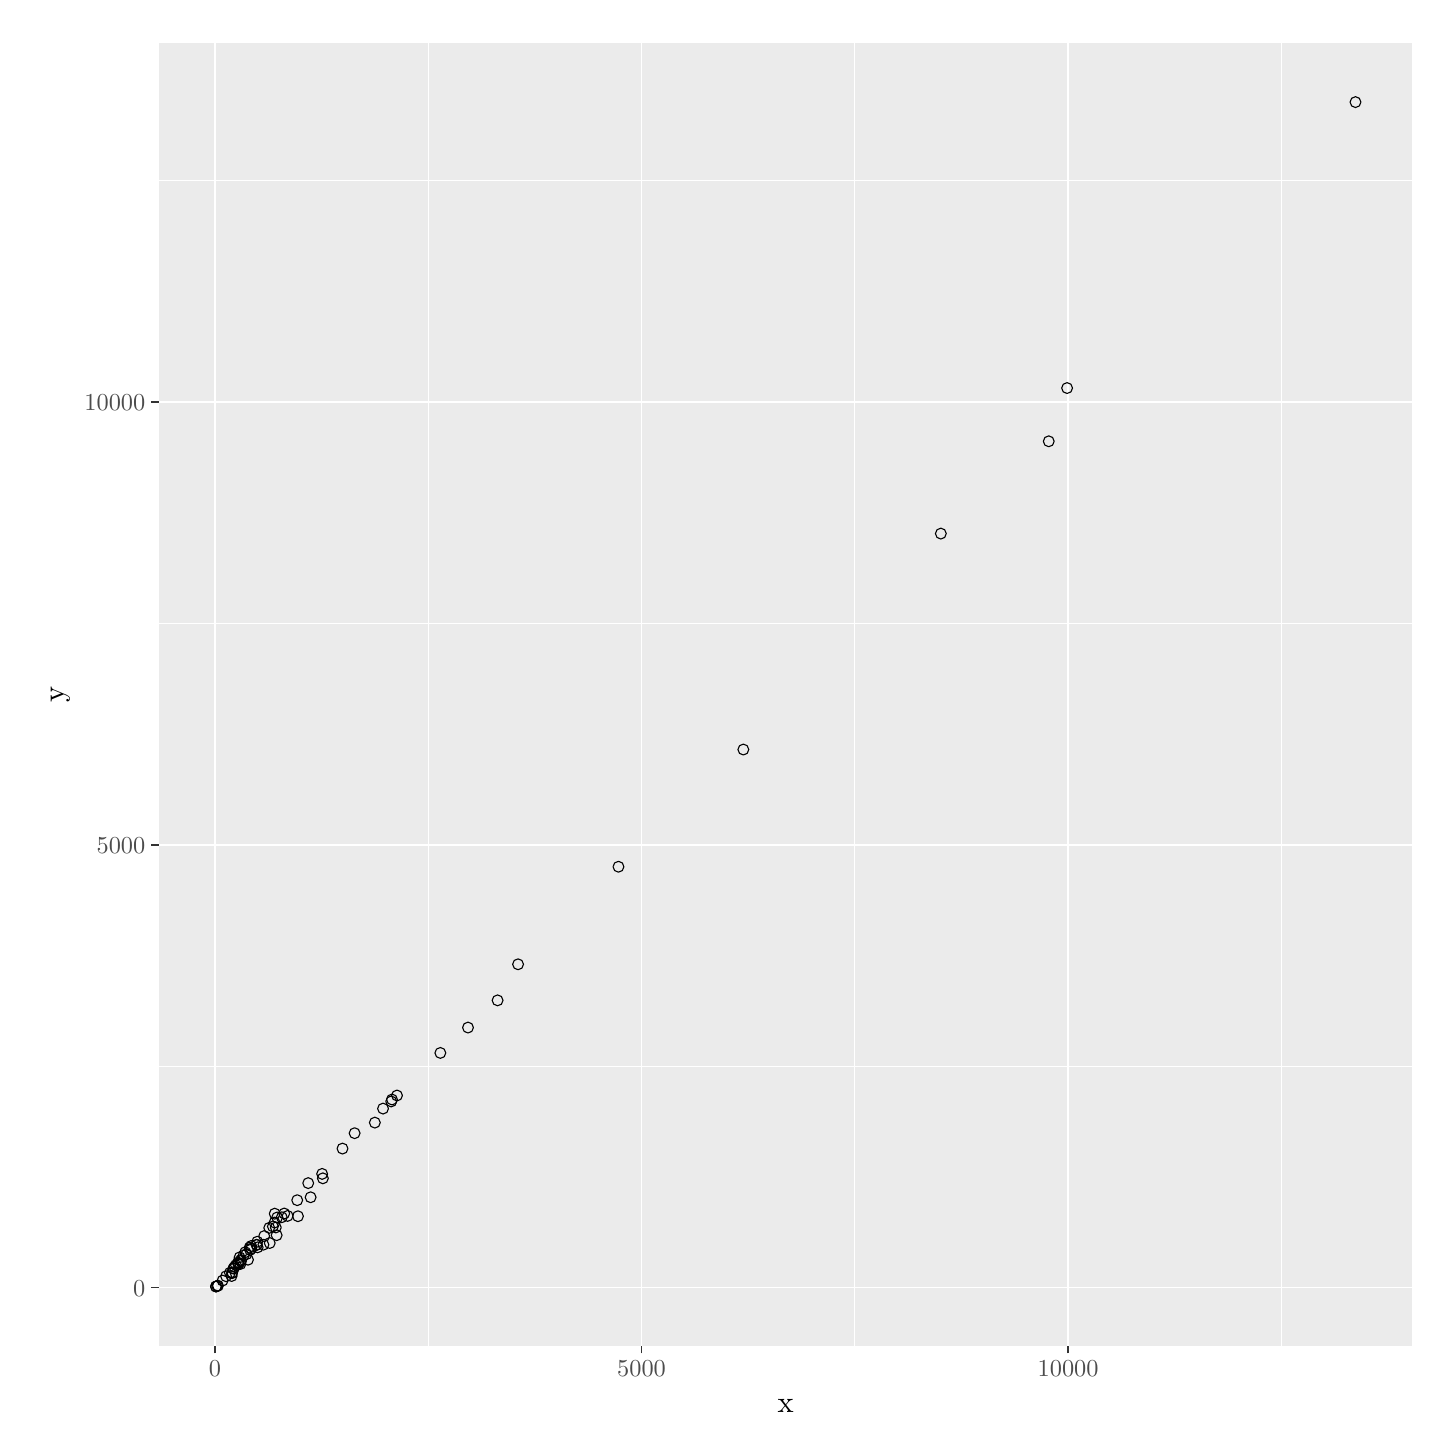
\begin{tikzpicture}[x=1pt,y=1pt]
\definecolor{fillColor}{RGB}{255,255,255}
\path[use as bounding box,fill=fillColor,fill opacity=0.00] (0,0) rectangle (505.89,505.89);
\begin{scope}
\path[clip] (  0.00,  0.00) rectangle (505.89,505.89);
\definecolor{drawColor}{RGB}{255,255,255}
\definecolor{fillColor}{RGB}{255,255,255}

\path[draw=drawColor,line width= 0.6pt,line join=round,line cap=round,fill=fillColor] (  0.00,  0.00) rectangle (505.89,505.89);
\end{scope}
\begin{scope}
\path[clip] ( 47.46, 29.59) rectangle (500.39,500.39);
\definecolor{fillColor}{gray}{0.92}

\path[fill=fillColor] ( 47.46, 29.59) rectangle (500.39,500.39);
\definecolor{drawColor}{RGB}{255,255,255}

\path[draw=drawColor,line width= 0.3pt,line join=round] ( 47.46,130.61) --
	(500.39,130.61);

\path[draw=drawColor,line width= 0.3pt,line join=round] ( 47.46,290.63) --
	(500.39,290.63);

\path[draw=drawColor,line width= 0.3pt,line join=round] ( 47.46,450.66) --
	(500.39,450.66);

\path[draw=drawColor,line width= 0.3pt,line join=round] (144.77, 29.59) --
	(144.77,500.39);

\path[draw=drawColor,line width= 0.3pt,line join=round] (298.89, 29.59) --
	(298.89,500.39);

\path[draw=drawColor,line width= 0.3pt,line join=round] (453.02, 29.59) --
	(453.02,500.39);

\path[draw=drawColor,line width= 0.6pt,line join=round] ( 47.46, 50.60) --
	(500.39, 50.60);

\path[draw=drawColor,line width= 0.6pt,line join=round] ( 47.46,210.62) --
	(500.39,210.62);

\path[draw=drawColor,line width= 0.6pt,line join=round] ( 47.46,370.64) --
	(500.39,370.64);

\path[draw=drawColor,line width= 0.6pt,line join=round] ( 67.71, 29.59) --
	( 67.71,500.39);

\path[draw=drawColor,line width= 0.6pt,line join=round] (221.83, 29.59) --
	(221.83,500.39);

\path[draw=drawColor,line width= 0.6pt,line join=round] (375.96, 29.59) --
	(375.96,500.39);
\definecolor{drawColor}{RGB}{0,0,0}

\path[draw=drawColor,line width= 0.4pt,line join=round,line cap=round] ( 68.05, 50.99) circle (  1.96);

\path[draw=drawColor,line width= 0.4pt,line join=round,line cap=round] ( 68.05, 50.99) circle (  1.96);

\path[draw=drawColor,line width= 0.4pt,line join=round,line cap=round] ( 68.48, 51.22) circle (  1.96);

\path[draw=drawColor,line width= 0.4pt,line join=round,line cap=round] ( 68.76, 51.31) circle (  1.96);

\path[draw=drawColor,line width= 0.4pt,line join=round,line cap=round] ( 70.43, 53.15) circle (  1.96);

\path[draw=drawColor,line width= 0.4pt,line join=round,line cap=round] ( 71.69, 54.72) circle (  1.96);

\path[draw=drawColor,line width= 0.4pt,line join=round,line cap=round] ( 73.08, 55.97) circle (  1.96);

\path[draw=drawColor,line width= 0.4pt,line join=round,line cap=round] ( 73.69, 54.80) circle (  1.96);

\path[draw=drawColor,line width= 0.4pt,line join=round,line cap=round] ( 73.85, 55.82) circle (  1.96);

\path[draw=drawColor,line width= 0.4pt,line join=round,line cap=round] ( 73.91, 56.10) circle (  1.96);

\path[draw=drawColor,line width= 0.4pt,line join=round,line cap=round] ( 74.37, 57.53) circle (  1.96);

\path[draw=drawColor,line width= 0.4pt,line join=round,line cap=round] ( 74.37, 57.53) circle (  1.96);

\path[draw=drawColor,line width= 0.4pt,line join=round,line cap=round] ( 74.74, 58.06) circle (  1.96);

\path[draw=drawColor,line width= 0.4pt,line join=round,line cap=round] ( 75.27, 58.75) circle (  1.96);

\path[draw=drawColor,line width= 0.4pt,line join=round,line cap=round] ( 76.00, 59.70) circle (  1.96);

\path[draw=drawColor,line width= 0.4pt,line join=round,line cap=round] ( 76.07, 59.24) circle (  1.96);

\path[draw=drawColor,line width= 0.4pt,line join=round,line cap=round] ( 76.28, 59.24) circle (  1.96);

\path[draw=drawColor,line width= 0.4pt,line join=round,line cap=round] ( 76.59, 61.55) circle (  1.96);

\path[draw=drawColor,line width= 0.4pt,line join=round,line cap=round] ( 76.87, 59.15) circle (  1.96);

\path[draw=drawColor,line width= 0.4pt,line join=round,line cap=round] ( 77.08, 60.63) circle (  1.96);

\path[draw=drawColor,line width= 0.4pt,line join=round,line cap=round] ( 77.11, 60.28) circle (  1.96);

\path[draw=drawColor,line width= 0.4pt,line join=round,line cap=round] ( 78.01, 62.20) circle (  1.96);

\path[draw=drawColor,line width= 0.4pt,line join=round,line cap=round] ( 78.62, 63.40) circle (  1.96);

\path[draw=drawColor,line width= 0.4pt,line join=round,line cap=round] ( 79.06, 62.70) circle (  1.96);

\path[draw=drawColor,line width= 0.4pt,line join=round,line cap=round] ( 79.61, 60.69) circle (  1.96);

\path[draw=drawColor,line width= 0.4pt,line join=round,line cap=round] ( 80.20, 65.06) circle (  1.96);

\path[draw=drawColor,line width= 0.4pt,line join=round,line cap=round] ( 80.38, 64.23) circle (  1.96);

\path[draw=drawColor,line width= 0.4pt,line join=round,line cap=round] ( 80.75, 65.65) circle (  1.96);

\path[draw=drawColor,line width= 0.4pt,line join=round,line cap=round] ( 80.81, 64.72) circle (  1.96);

\path[draw=drawColor,line width= 0.4pt,line join=round,line cap=round] ( 82.76, 66.06) circle (  1.96);

\path[draw=drawColor,line width= 0.4pt,line join=round,line cap=round] ( 82.76, 66.06) circle (  1.96);

\path[draw=drawColor,line width= 0.4pt,line join=round,line cap=round] ( 82.97, 67.20) circle (  1.96);

\path[draw=drawColor,line width= 0.4pt,line join=round,line cap=round] ( 83.09, 65.17) circle (  1.96);

\path[draw=drawColor,line width= 0.4pt,line join=round,line cap=round] ( 85.19, 66.12) circle (  1.96);

\path[draw=drawColor,line width= 0.4pt,line join=round,line cap=round] ( 85.47, 69.24) circle (  1.96);

\path[draw=drawColor,line width= 0.4pt,line join=round,line cap=round] ( 87.29, 72.20) circle (  1.96);

\path[draw=drawColor,line width= 0.4pt,line join=round,line cap=round] ( 87.47, 66.72) circle (  1.96);

\path[draw=drawColor,line width= 0.4pt,line join=round,line cap=round] ( 88.61, 72.70) circle (  1.96);

\path[draw=drawColor,line width= 0.4pt,line join=round,line cap=round] ( 89.20, 74.12) circle (  1.96);

\path[draw=drawColor,line width= 0.4pt,line join=round,line cap=round] ( 89.26, 77.33) circle (  1.96);

\path[draw=drawColor,line width= 0.4pt,line join=round,line cap=round] ( 89.66, 72.34) circle (  1.96);

\path[draw=drawColor,line width= 0.4pt,line join=round,line cap=round] ( 89.97, 69.55) circle (  1.96);

\path[draw=drawColor,line width= 0.4pt,line join=round,line cap=round] ( 90.15, 75.96) circle (  1.96);

\path[draw=drawColor,line width= 0.4pt,line join=round,line cap=round] ( 91.82, 76.03) circle (  1.96);

\path[draw=drawColor,line width= 0.4pt,line join=round,line cap=round] ( 92.71, 77.39) circle (  1.96);

\path[draw=drawColor,line width= 0.4pt,line join=round,line cap=round] ( 93.94, 76.52) circle (  1.96);

\path[draw=drawColor,line width= 0.4pt,line join=round,line cap=round] ( 97.40, 82.20) circle (  1.96);

\path[draw=drawColor,line width= 0.4pt,line join=round,line cap=round] ( 97.67, 76.40) circle (  1.96);

\path[draw=drawColor,line width= 0.4pt,line join=round,line cap=round] (101.37, 88.37) circle (  1.96);

\path[draw=drawColor,line width= 0.4pt,line join=round,line cap=round] (102.24, 83.25) circle (  1.96);

\path[draw=drawColor,line width= 0.4pt,line join=round,line cap=round] (106.40, 91.70) circle (  1.96);

\path[draw=drawColor,line width= 0.4pt,line join=round,line cap=round] (106.67, 90.10) circle (  1.96);

\path[draw=drawColor,line width= 0.4pt,line join=round,line cap=round] (113.76,100.85) circle (  1.96);

\path[draw=drawColor,line width= 0.4pt,line join=round,line cap=round] (118.14,106.41) circle (  1.96);

\path[draw=drawColor,line width= 0.4pt,line join=round,line cap=round] (125.45,110.23) circle (  1.96);

\path[draw=drawColor,line width= 0.4pt,line join=round,line cap=round] (128.41,115.30) circle (  1.96);

\path[draw=drawColor,line width= 0.4pt,line join=round,line cap=round] (131.37,117.88) circle (  1.96);

\path[draw=drawColor,line width= 0.4pt,line join=round,line cap=round] (131.64,118.58) circle (  1.96);

\path[draw=drawColor,line width= 0.4pt,line join=round,line cap=round] (133.46,120.03) circle (  1.96);

\path[draw=drawColor,line width= 0.4pt,line join=round,line cap=round] (149.12,135.41) circle (  1.96);

\path[draw=drawColor,line width= 0.4pt,line join=round,line cap=round] (159.11,144.58) circle (  1.96);

\path[draw=drawColor,line width= 0.4pt,line join=round,line cap=round] (169.80,154.41) circle (  1.96);

\path[draw=drawColor,line width= 0.4pt,line join=round,line cap=round] (177.20,167.44) circle (  1.96);

\path[draw=drawColor,line width= 0.4pt,line join=round,line cap=round] (213.48,202.69) circle (  1.96);

\path[draw=drawColor,line width= 0.4pt,line join=round,line cap=round] (258.61,245.04) circle (  1.96);

\path[draw=drawColor,line width= 0.4pt,line join=round,line cap=round] (329.97,323.07) circle (  1.96);

\path[draw=drawColor,line width= 0.4pt,line join=round,line cap=round] (368.96,356.42) circle (  1.96);

\path[draw=drawColor,line width= 0.4pt,line join=round,line cap=round] (375.59,375.66) circle (  1.96);

\path[draw=drawColor,line width= 0.4pt,line join=round,line cap=round] (479.80,478.99) circle (  1.96);
\end{scope}
\begin{scope}
\path[clip] (  0.00,  0.00) rectangle (505.89,505.89);
\definecolor{drawColor}{gray}{0.30}

\node[text=drawColor,anchor=base east,inner sep=0pt, outer sep=0pt, scale=  0.88] at ( 42.51, 47.57) {0};

\node[text=drawColor,anchor=base east,inner sep=0pt, outer sep=0pt, scale=  0.88] at ( 42.51,207.59) {5000};

\node[text=drawColor,anchor=base east,inner sep=0pt, outer sep=0pt, scale=  0.88] at ( 42.51,367.61) {10000};
\end{scope}
\begin{scope}
\path[clip] (  0.00,  0.00) rectangle (505.89,505.89);
\definecolor{drawColor}{gray}{0.20}

\path[draw=drawColor,line width= 0.6pt,line join=round] ( 44.71, 50.60) --
	( 47.46, 50.60);

\path[draw=drawColor,line width= 0.6pt,line join=round] ( 44.71,210.62) --
	( 47.46,210.62);

\path[draw=drawColor,line width= 0.6pt,line join=round] ( 44.71,370.64) --
	( 47.46,370.64);
\end{scope}
\begin{scope}
\path[clip] (  0.00,  0.00) rectangle (505.89,505.89);
\definecolor{drawColor}{gray}{0.20}

\path[draw=drawColor,line width= 0.6pt,line join=round] ( 67.71, 26.84) --
	( 67.71, 29.59);

\path[draw=drawColor,line width= 0.6pt,line join=round] (221.83, 26.84) --
	(221.83, 29.59);

\path[draw=drawColor,line width= 0.6pt,line join=round] (375.96, 26.84) --
	(375.96, 29.59);
\end{scope}
\begin{scope}
\path[clip] (  0.00,  0.00) rectangle (505.89,505.89);
\definecolor{drawColor}{gray}{0.30}

\node[text=drawColor,anchor=base,inner sep=0pt, outer sep=0pt, scale=  0.88] at ( 67.71, 18.58) {0};

\node[text=drawColor,anchor=base,inner sep=0pt, outer sep=0pt, scale=  0.88] at (221.83, 18.58) {5000};

\node[text=drawColor,anchor=base,inner sep=0pt, outer sep=0pt, scale=  0.88] at (375.96, 18.58) {10000};
\end{scope}
\begin{scope}
\path[clip] (  0.00,  0.00) rectangle (505.89,505.89);
\definecolor{drawColor}{RGB}{0,0,0}

\node[text=drawColor,anchor=base,inner sep=0pt, outer sep=0pt, scale=  1.10] at (273.93,  5.50) {x};
\end{scope}
\begin{scope}
\path[clip] (  0.00,  0.00) rectangle (505.89,505.89);
\definecolor{drawColor}{RGB}{0,0,0}

\node[text=drawColor,rotate= 90.00,anchor=base,inner sep=0pt, outer sep=0pt, scale=  1.10] at ( 13.08,264.99) {y};
\end{scope}
\end{tikzpicture}
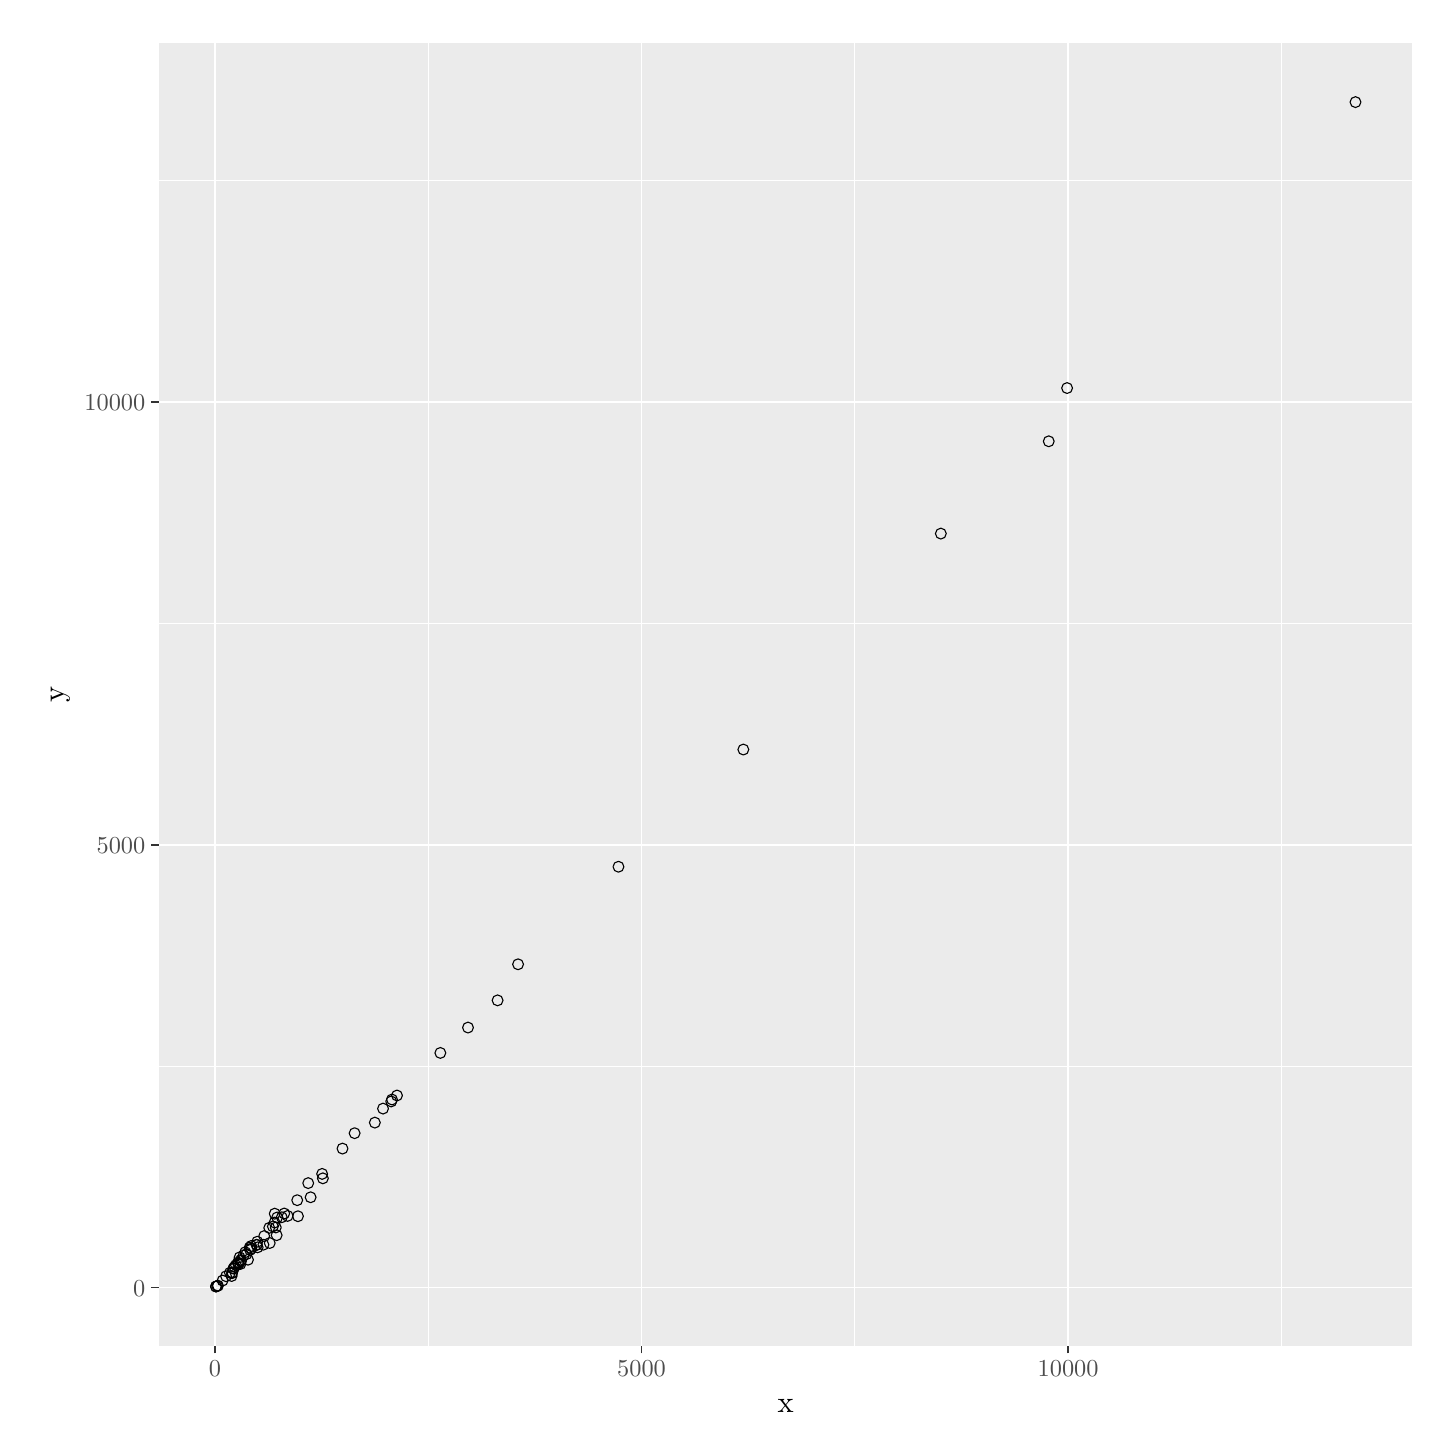
\begin{tikzpicture}[x=1pt,y=1pt]
\definecolor{fillColor}{RGB}{255,255,255}
\path[use as bounding box,fill=fillColor,fill opacity=0.00] (0,0) rectangle (505.89,505.89);
\begin{scope}
\path[clip] (  0.00,  0.00) rectangle (505.89,505.89);
\definecolor{drawColor}{RGB}{255,255,255}
\definecolor{fillColor}{RGB}{255,255,255}

\path[draw=drawColor,line width= 0.6pt,line join=round,line cap=round,fill=fillColor] (  0.00,  0.00) rectangle (505.89,505.89);
\end{scope}
\begin{scope}
\path[clip] ( 47.46, 29.59) rectangle (500.39,500.39);
\definecolor{fillColor}{gray}{0.92}

\path[fill=fillColor] ( 47.46, 29.59) rectangle (500.39,500.39);
\definecolor{drawColor}{RGB}{255,255,255}

\path[draw=drawColor,line width= 0.3pt,line join=round] ( 47.46,130.61) --
	(500.39,130.61);

\path[draw=drawColor,line width= 0.3pt,line join=round] ( 47.46,290.63) --
	(500.39,290.63);

\path[draw=drawColor,line width= 0.3pt,line join=round] ( 47.46,450.66) --
	(500.39,450.66);

\path[draw=drawColor,line width= 0.3pt,line join=round] (144.77, 29.59) --
	(144.77,500.39);

\path[draw=drawColor,line width= 0.3pt,line join=round] (298.89, 29.59) --
	(298.89,500.39);

\path[draw=drawColor,line width= 0.3pt,line join=round] (453.02, 29.59) --
	(453.02,500.39);

\path[draw=drawColor,line width= 0.6pt,line join=round] ( 47.46, 50.60) --
	(500.39, 50.60);

\path[draw=drawColor,line width= 0.6pt,line join=round] ( 47.46,210.62) --
	(500.39,210.62);

\path[draw=drawColor,line width= 0.6pt,line join=round] ( 47.46,370.64) --
	(500.39,370.64);

\path[draw=drawColor,line width= 0.6pt,line join=round] ( 67.71, 29.59) --
	( 67.71,500.39);

\path[draw=drawColor,line width= 0.6pt,line join=round] (221.83, 29.59) --
	(221.83,500.39);

\path[draw=drawColor,line width= 0.6pt,line join=round] (375.96, 29.59) --
	(375.96,500.39);
\definecolor{drawColor}{RGB}{0,0,0}

\path[draw=drawColor,line width= 0.4pt,line join=round,line cap=round] ( 68.05, 50.99) circle (  1.96);

\path[draw=drawColor,line width= 0.4pt,line join=round,line cap=round] ( 68.05, 50.99) circle (  1.96);

\path[draw=drawColor,line width= 0.4pt,line join=round,line cap=round] ( 68.48, 51.22) circle (  1.96);

\path[draw=drawColor,line width= 0.4pt,line join=round,line cap=round] ( 68.76, 51.31) circle (  1.96);

\path[draw=drawColor,line width= 0.4pt,line join=round,line cap=round] ( 70.43, 53.15) circle (  1.96);

\path[draw=drawColor,line width= 0.4pt,line join=round,line cap=round] ( 71.69, 54.72) circle (  1.96);

\path[draw=drawColor,line width= 0.4pt,line join=round,line cap=round] ( 73.08, 55.97) circle (  1.96);

\path[draw=drawColor,line width= 0.4pt,line join=round,line cap=round] ( 73.69, 54.80) circle (  1.96);

\path[draw=drawColor,line width= 0.4pt,line join=round,line cap=round] ( 73.85, 55.82) circle (  1.96);

\path[draw=drawColor,line width= 0.4pt,line join=round,line cap=round] ( 73.91, 56.10) circle (  1.96);

\path[draw=drawColor,line width= 0.4pt,line join=round,line cap=round] ( 74.37, 57.53) circle (  1.96);

\path[draw=drawColor,line width= 0.4pt,line join=round,line cap=round] ( 74.37, 57.53) circle (  1.96);

\path[draw=drawColor,line width= 0.4pt,line join=round,line cap=round] ( 74.74, 58.06) circle (  1.96);

\path[draw=drawColor,line width= 0.4pt,line join=round,line cap=round] ( 75.27, 58.75) circle (  1.96);

\path[draw=drawColor,line width= 0.4pt,line join=round,line cap=round] ( 76.00, 59.70) circle (  1.96);

\path[draw=drawColor,line width= 0.4pt,line join=round,line cap=round] ( 76.07, 59.24) circle (  1.96);

\path[draw=drawColor,line width= 0.4pt,line join=round,line cap=round] ( 76.28, 59.24) circle (  1.96);

\path[draw=drawColor,line width= 0.4pt,line join=round,line cap=round] ( 76.59, 61.55) circle (  1.96);

\path[draw=drawColor,line width= 0.4pt,line join=round,line cap=round] ( 76.87, 59.15) circle (  1.96);

\path[draw=drawColor,line width= 0.4pt,line join=round,line cap=round] ( 77.08, 60.63) circle (  1.96);

\path[draw=drawColor,line width= 0.4pt,line join=round,line cap=round] ( 77.11, 60.28) circle (  1.96);

\path[draw=drawColor,line width= 0.4pt,line join=round,line cap=round] ( 78.01, 62.20) circle (  1.96);

\path[draw=drawColor,line width= 0.4pt,line join=round,line cap=round] ( 78.62, 63.40) circle (  1.96);

\path[draw=drawColor,line width= 0.4pt,line join=round,line cap=round] ( 79.06, 62.70) circle (  1.96);

\path[draw=drawColor,line width= 0.4pt,line join=round,line cap=round] ( 79.61, 60.69) circle (  1.96);

\path[draw=drawColor,line width= 0.4pt,line join=round,line cap=round] ( 80.20, 65.06) circle (  1.96);

\path[draw=drawColor,line width= 0.4pt,line join=round,line cap=round] ( 80.38, 64.23) circle (  1.96);

\path[draw=drawColor,line width= 0.4pt,line join=round,line cap=round] ( 80.75, 65.65) circle (  1.96);

\path[draw=drawColor,line width= 0.4pt,line join=round,line cap=round] ( 80.81, 64.72) circle (  1.96);

\path[draw=drawColor,line width= 0.4pt,line join=round,line cap=round] ( 82.76, 66.06) circle (  1.96);

\path[draw=drawColor,line width= 0.4pt,line join=round,line cap=round] ( 82.76, 66.06) circle (  1.96);

\path[draw=drawColor,line width= 0.4pt,line join=round,line cap=round] ( 82.97, 67.20) circle (  1.96);

\path[draw=drawColor,line width= 0.4pt,line join=round,line cap=round] ( 83.09, 65.17) circle (  1.96);

\path[draw=drawColor,line width= 0.4pt,line join=round,line cap=round] ( 85.19, 66.12) circle (  1.96);

\path[draw=drawColor,line width= 0.4pt,line join=round,line cap=round] ( 85.47, 69.24) circle (  1.96);

\path[draw=drawColor,line width= 0.4pt,line join=round,line cap=round] ( 87.29, 72.20) circle (  1.96);

\path[draw=drawColor,line width= 0.4pt,line join=round,line cap=round] ( 87.47, 66.72) circle (  1.96);

\path[draw=drawColor,line width= 0.4pt,line join=round,line cap=round] ( 88.61, 72.70) circle (  1.96);

\path[draw=drawColor,line width= 0.4pt,line join=round,line cap=round] ( 89.20, 74.12) circle (  1.96);

\path[draw=drawColor,line width= 0.4pt,line join=round,line cap=round] ( 89.26, 77.33) circle (  1.96);

\path[draw=drawColor,line width= 0.4pt,line join=round,line cap=round] ( 89.66, 72.34) circle (  1.96);

\path[draw=drawColor,line width= 0.4pt,line join=round,line cap=round] ( 89.97, 69.55) circle (  1.96);

\path[draw=drawColor,line width= 0.4pt,line join=round,line cap=round] ( 90.15, 75.96) circle (  1.96);

\path[draw=drawColor,line width= 0.4pt,line join=round,line cap=round] ( 91.82, 76.03) circle (  1.96);

\path[draw=drawColor,line width= 0.4pt,line join=round,line cap=round] ( 92.71, 77.39) circle (  1.96);

\path[draw=drawColor,line width= 0.4pt,line join=round,line cap=round] ( 93.94, 76.52) circle (  1.96);

\path[draw=drawColor,line width= 0.4pt,line join=round,line cap=round] ( 97.40, 82.20) circle (  1.96);

\path[draw=drawColor,line width= 0.4pt,line join=round,line cap=round] ( 97.67, 76.40) circle (  1.96);

\path[draw=drawColor,line width= 0.4pt,line join=round,line cap=round] (101.37, 88.37) circle (  1.96);

\path[draw=drawColor,line width= 0.4pt,line join=round,line cap=round] (102.24, 83.25) circle (  1.96);

\path[draw=drawColor,line width= 0.4pt,line join=round,line cap=round] (106.40, 91.70) circle (  1.96);

\path[draw=drawColor,line width= 0.4pt,line join=round,line cap=round] (106.67, 90.10) circle (  1.96);

\path[draw=drawColor,line width= 0.4pt,line join=round,line cap=round] (113.76,100.85) circle (  1.96);

\path[draw=drawColor,line width= 0.4pt,line join=round,line cap=round] (118.14,106.41) circle (  1.96);

\path[draw=drawColor,line width= 0.4pt,line join=round,line cap=round] (125.45,110.23) circle (  1.96);

\path[draw=drawColor,line width= 0.4pt,line join=round,line cap=round] (128.41,115.30) circle (  1.96);

\path[draw=drawColor,line width= 0.4pt,line join=round,line cap=round] (131.37,117.88) circle (  1.96);

\path[draw=drawColor,line width= 0.4pt,line join=round,line cap=round] (131.64,118.58) circle (  1.96);

\path[draw=drawColor,line width= 0.4pt,line join=round,line cap=round] (133.46,120.03) circle (  1.96);

\path[draw=drawColor,line width= 0.4pt,line join=round,line cap=round] (149.12,135.41) circle (  1.96);

\path[draw=drawColor,line width= 0.4pt,line join=round,line cap=round] (159.11,144.58) circle (  1.96);

\path[draw=drawColor,line width= 0.4pt,line join=round,line cap=round] (169.80,154.41) circle (  1.96);

\path[draw=drawColor,line width= 0.4pt,line join=round,line cap=round] (177.20,167.44) circle (  1.96);

\path[draw=drawColor,line width= 0.4pt,line join=round,line cap=round] (213.48,202.69) circle (  1.96);

\path[draw=drawColor,line width= 0.4pt,line join=round,line cap=round] (258.61,245.04) circle (  1.96);

\path[draw=drawColor,line width= 0.4pt,line join=round,line cap=round] (329.97,323.07) circle (  1.96);

\path[draw=drawColor,line width= 0.4pt,line join=round,line cap=round] (368.96,356.42) circle (  1.96);

\path[draw=drawColor,line width= 0.4pt,line join=round,line cap=round] (375.59,375.66) circle (  1.96);

\path[draw=drawColor,line width= 0.4pt,line join=round,line cap=round] (479.80,478.99) circle (  1.96);
\end{scope}
\begin{scope}
\path[clip] (  0.00,  0.00) rectangle (505.89,505.89);
\definecolor{drawColor}{gray}{0.30}

\node[text=drawColor,anchor=base east,inner sep=0pt, outer sep=0pt, scale=  0.88] at ( 42.51, 47.57) {0};

\node[text=drawColor,anchor=base east,inner sep=0pt, outer sep=0pt, scale=  0.88] at ( 42.51,207.59) {5000};

\node[text=drawColor,anchor=base east,inner sep=0pt, outer sep=0pt, scale=  0.88] at ( 42.51,367.61) {10000};
\end{scope}
\begin{scope}
\path[clip] (  0.00,  0.00) rectangle (505.89,505.89);
\definecolor{drawColor}{gray}{0.20}

\path[draw=drawColor,line width= 0.6pt,line join=round] ( 44.71, 50.60) --
	( 47.46, 50.60);

\path[draw=drawColor,line width= 0.6pt,line join=round] ( 44.71,210.62) --
	( 47.46,210.62);

\path[draw=drawColor,line width= 0.6pt,line join=round] ( 44.71,370.64) --
	( 47.46,370.64);
\end{scope}
\begin{scope}
\path[clip] (  0.00,  0.00) rectangle (505.89,505.89);
\definecolor{drawColor}{gray}{0.20}

\path[draw=drawColor,line width= 0.6pt,line join=round] ( 67.71, 26.84) --
	( 67.71, 29.59);

\path[draw=drawColor,line width= 0.6pt,line join=round] (221.83, 26.84) --
	(221.83, 29.59);

\path[draw=drawColor,line width= 0.6pt,line join=round] (375.96, 26.84) --
	(375.96, 29.59);
\end{scope}
\begin{scope}
\path[clip] (  0.00,  0.00) rectangle (505.89,505.89);
\definecolor{drawColor}{gray}{0.30}

\node[text=drawColor,anchor=base,inner sep=0pt, outer sep=0pt, scale=  0.88] at ( 67.71, 18.58) {0};

\node[text=drawColor,anchor=base,inner sep=0pt, outer sep=0pt, scale=  0.88] at (221.83, 18.58) {5000};

\node[text=drawColor,anchor=base,inner sep=0pt, outer sep=0pt, scale=  0.88] at (375.96, 18.58) {10000};
\end{scope}
\begin{scope}
\path[clip] (  0.00,  0.00) rectangle (505.89,505.89);
\definecolor{drawColor}{RGB}{0,0,0}

\node[text=drawColor,anchor=base,inner sep=0pt, outer sep=0pt, scale=  1.10] at (273.93,  5.50) {x};
\end{scope}
\begin{scope}
\path[clip] (  0.00,  0.00) rectangle (505.89,505.89);
\definecolor{drawColor}{RGB}{0,0,0}

\node[text=drawColor,rotate= 90.00,anchor=base,inner sep=0pt, outer sep=0pt, scale=  1.10] at ( 13.08,264.99) {y};
\end{scope}
\end{tikzpicture}
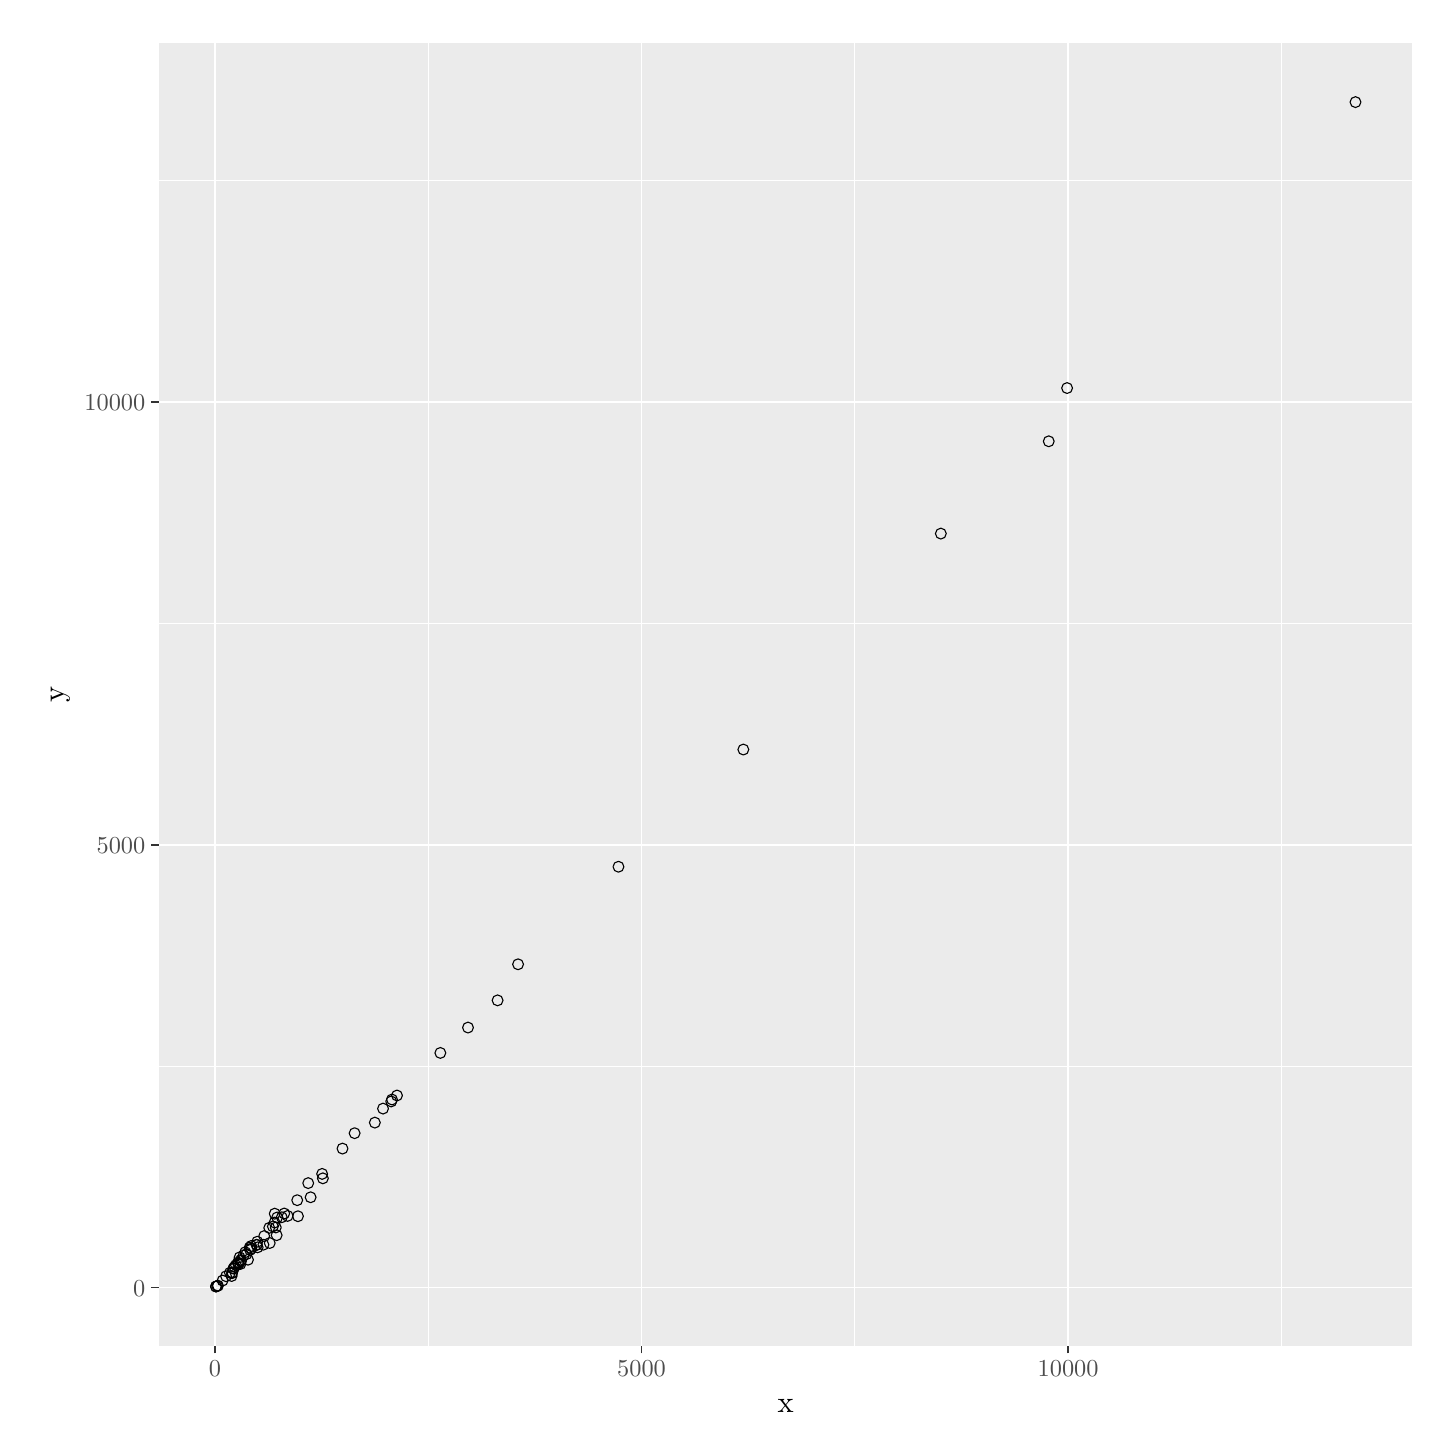
\begin{tikzpicture}[x=1pt,y=1pt]
\definecolor{fillColor}{RGB}{255,255,255}
\path[use as bounding box,fill=fillColor,fill opacity=0.00] (0,0) rectangle (505.89,505.89);
\begin{scope}
\path[clip] (  0.00,  0.00) rectangle (505.89,505.89);
\definecolor{drawColor}{RGB}{255,255,255}
\definecolor{fillColor}{RGB}{255,255,255}

\path[draw=drawColor,line width= 0.6pt,line join=round,line cap=round,fill=fillColor] (  0.00,  0.00) rectangle (505.89,505.89);
\end{scope}
\begin{scope}
\path[clip] ( 47.46, 29.59) rectangle (500.39,500.39);
\definecolor{fillColor}{gray}{0.92}

\path[fill=fillColor] ( 47.46, 29.59) rectangle (500.39,500.39);
\definecolor{drawColor}{RGB}{255,255,255}

\path[draw=drawColor,line width= 0.3pt,line join=round] ( 47.46,130.61) --
	(500.39,130.61);

\path[draw=drawColor,line width= 0.3pt,line join=round] ( 47.46,290.63) --
	(500.39,290.63);

\path[draw=drawColor,line width= 0.3pt,line join=round] ( 47.46,450.66) --
	(500.39,450.66);

\path[draw=drawColor,line width= 0.3pt,line join=round] (144.77, 29.59) --
	(144.77,500.39);

\path[draw=drawColor,line width= 0.3pt,line join=round] (298.89, 29.59) --
	(298.89,500.39);

\path[draw=drawColor,line width= 0.3pt,line join=round] (453.02, 29.59) --
	(453.02,500.39);

\path[draw=drawColor,line width= 0.6pt,line join=round] ( 47.46, 50.60) --
	(500.39, 50.60);

\path[draw=drawColor,line width= 0.6pt,line join=round] ( 47.46,210.62) --
	(500.39,210.62);

\path[draw=drawColor,line width= 0.6pt,line join=round] ( 47.46,370.64) --
	(500.39,370.64);

\path[draw=drawColor,line width= 0.6pt,line join=round] ( 67.71, 29.59) --
	( 67.71,500.39);

\path[draw=drawColor,line width= 0.6pt,line join=round] (221.83, 29.59) --
	(221.83,500.39);

\path[draw=drawColor,line width= 0.6pt,line join=round] (375.96, 29.59) --
	(375.96,500.39);
\definecolor{drawColor}{RGB}{0,0,0}

\path[draw=drawColor,line width= 0.4pt,line join=round,line cap=round] ( 68.05, 50.99) circle (  1.96);

\path[draw=drawColor,line width= 0.4pt,line join=round,line cap=round] ( 68.05, 50.99) circle (  1.96);

\path[draw=drawColor,line width= 0.4pt,line join=round,line cap=round] ( 68.48, 51.22) circle (  1.96);

\path[draw=drawColor,line width= 0.4pt,line join=round,line cap=round] ( 68.76, 51.31) circle (  1.96);

\path[draw=drawColor,line width= 0.4pt,line join=round,line cap=round] ( 70.43, 53.15) circle (  1.96);

\path[draw=drawColor,line width= 0.4pt,line join=round,line cap=round] ( 71.69, 54.72) circle (  1.96);

\path[draw=drawColor,line width= 0.4pt,line join=round,line cap=round] ( 73.08, 55.97) circle (  1.96);

\path[draw=drawColor,line width= 0.4pt,line join=round,line cap=round] ( 73.69, 54.80) circle (  1.96);

\path[draw=drawColor,line width= 0.4pt,line join=round,line cap=round] ( 73.85, 55.82) circle (  1.96);

\path[draw=drawColor,line width= 0.4pt,line join=round,line cap=round] ( 73.91, 56.10) circle (  1.96);

\path[draw=drawColor,line width= 0.4pt,line join=round,line cap=round] ( 74.37, 57.53) circle (  1.96);

\path[draw=drawColor,line width= 0.4pt,line join=round,line cap=round] ( 74.37, 57.53) circle (  1.96);

\path[draw=drawColor,line width= 0.4pt,line join=round,line cap=round] ( 74.74, 58.06) circle (  1.96);

\path[draw=drawColor,line width= 0.4pt,line join=round,line cap=round] ( 75.27, 58.75) circle (  1.96);

\path[draw=drawColor,line width= 0.4pt,line join=round,line cap=round] ( 76.00, 59.70) circle (  1.96);

\path[draw=drawColor,line width= 0.4pt,line join=round,line cap=round] ( 76.07, 59.24) circle (  1.96);

\path[draw=drawColor,line width= 0.4pt,line join=round,line cap=round] ( 76.28, 59.24) circle (  1.96);

\path[draw=drawColor,line width= 0.4pt,line join=round,line cap=round] ( 76.59, 61.55) circle (  1.96);

\path[draw=drawColor,line width= 0.4pt,line join=round,line cap=round] ( 76.87, 59.15) circle (  1.96);

\path[draw=drawColor,line width= 0.4pt,line join=round,line cap=round] ( 77.08, 60.63) circle (  1.96);

\path[draw=drawColor,line width= 0.4pt,line join=round,line cap=round] ( 77.11, 60.28) circle (  1.96);

\path[draw=drawColor,line width= 0.4pt,line join=round,line cap=round] ( 78.01, 62.20) circle (  1.96);

\path[draw=drawColor,line width= 0.4pt,line join=round,line cap=round] ( 78.62, 63.40) circle (  1.96);

\path[draw=drawColor,line width= 0.4pt,line join=round,line cap=round] ( 79.06, 62.70) circle (  1.96);

\path[draw=drawColor,line width= 0.4pt,line join=round,line cap=round] ( 79.61, 60.69) circle (  1.96);

\path[draw=drawColor,line width= 0.4pt,line join=round,line cap=round] ( 80.20, 65.06) circle (  1.96);

\path[draw=drawColor,line width= 0.4pt,line join=round,line cap=round] ( 80.38, 64.23) circle (  1.96);

\path[draw=drawColor,line width= 0.4pt,line join=round,line cap=round] ( 80.75, 65.65) circle (  1.96);

\path[draw=drawColor,line width= 0.4pt,line join=round,line cap=round] ( 80.81, 64.72) circle (  1.96);

\path[draw=drawColor,line width= 0.4pt,line join=round,line cap=round] ( 82.76, 66.06) circle (  1.96);

\path[draw=drawColor,line width= 0.4pt,line join=round,line cap=round] ( 82.76, 66.06) circle (  1.96);

\path[draw=drawColor,line width= 0.4pt,line join=round,line cap=round] ( 82.97, 67.20) circle (  1.96);

\path[draw=drawColor,line width= 0.4pt,line join=round,line cap=round] ( 83.09, 65.17) circle (  1.96);

\path[draw=drawColor,line width= 0.4pt,line join=round,line cap=round] ( 85.19, 66.12) circle (  1.96);

\path[draw=drawColor,line width= 0.4pt,line join=round,line cap=round] ( 85.47, 69.24) circle (  1.96);

\path[draw=drawColor,line width= 0.4pt,line join=round,line cap=round] ( 87.29, 72.20) circle (  1.96);

\path[draw=drawColor,line width= 0.4pt,line join=round,line cap=round] ( 87.47, 66.72) circle (  1.96);

\path[draw=drawColor,line width= 0.4pt,line join=round,line cap=round] ( 88.61, 72.70) circle (  1.96);

\path[draw=drawColor,line width= 0.4pt,line join=round,line cap=round] ( 89.20, 74.12) circle (  1.96);

\path[draw=drawColor,line width= 0.4pt,line join=round,line cap=round] ( 89.26, 77.33) circle (  1.96);

\path[draw=drawColor,line width= 0.4pt,line join=round,line cap=round] ( 89.66, 72.34) circle (  1.96);

\path[draw=drawColor,line width= 0.4pt,line join=round,line cap=round] ( 89.97, 69.55) circle (  1.96);

\path[draw=drawColor,line width= 0.4pt,line join=round,line cap=round] ( 90.15, 75.96) circle (  1.96);

\path[draw=drawColor,line width= 0.4pt,line join=round,line cap=round] ( 91.82, 76.03) circle (  1.96);

\path[draw=drawColor,line width= 0.4pt,line join=round,line cap=round] ( 92.71, 77.39) circle (  1.96);

\path[draw=drawColor,line width= 0.4pt,line join=round,line cap=round] ( 93.94, 76.52) circle (  1.96);

\path[draw=drawColor,line width= 0.4pt,line join=round,line cap=round] ( 97.40, 82.20) circle (  1.96);

\path[draw=drawColor,line width= 0.4pt,line join=round,line cap=round] ( 97.67, 76.40) circle (  1.96);

\path[draw=drawColor,line width= 0.4pt,line join=round,line cap=round] (101.37, 88.37) circle (  1.96);

\path[draw=drawColor,line width= 0.4pt,line join=round,line cap=round] (102.24, 83.25) circle (  1.96);

\path[draw=drawColor,line width= 0.4pt,line join=round,line cap=round] (106.40, 91.70) circle (  1.96);

\path[draw=drawColor,line width= 0.4pt,line join=round,line cap=round] (106.67, 90.10) circle (  1.96);

\path[draw=drawColor,line width= 0.4pt,line join=round,line cap=round] (113.76,100.85) circle (  1.96);

\path[draw=drawColor,line width= 0.4pt,line join=round,line cap=round] (118.14,106.41) circle (  1.96);

\path[draw=drawColor,line width= 0.4pt,line join=round,line cap=round] (125.45,110.23) circle (  1.96);

\path[draw=drawColor,line width= 0.4pt,line join=round,line cap=round] (128.41,115.30) circle (  1.96);

\path[draw=drawColor,line width= 0.4pt,line join=round,line cap=round] (131.37,117.88) circle (  1.96);

\path[draw=drawColor,line width= 0.4pt,line join=round,line cap=round] (131.64,118.58) circle (  1.96);

\path[draw=drawColor,line width= 0.4pt,line join=round,line cap=round] (133.46,120.03) circle (  1.96);

\path[draw=drawColor,line width= 0.4pt,line join=round,line cap=round] (149.12,135.41) circle (  1.96);

\path[draw=drawColor,line width= 0.4pt,line join=round,line cap=round] (159.11,144.58) circle (  1.96);

\path[draw=drawColor,line width= 0.4pt,line join=round,line cap=round] (169.80,154.41) circle (  1.96);

\path[draw=drawColor,line width= 0.4pt,line join=round,line cap=round] (177.20,167.44) circle (  1.96);

\path[draw=drawColor,line width= 0.4pt,line join=round,line cap=round] (213.48,202.69) circle (  1.96);

\path[draw=drawColor,line width= 0.4pt,line join=round,line cap=round] (258.61,245.04) circle (  1.96);

\path[draw=drawColor,line width= 0.4pt,line join=round,line cap=round] (329.97,323.07) circle (  1.96);

\path[draw=drawColor,line width= 0.4pt,line join=round,line cap=round] (368.96,356.42) circle (  1.96);

\path[draw=drawColor,line width= 0.4pt,line join=round,line cap=round] (375.59,375.66) circle (  1.96);

\path[draw=drawColor,line width= 0.4pt,line join=round,line cap=round] (479.80,478.99) circle (  1.96);
\end{scope}
\begin{scope}
\path[clip] (  0.00,  0.00) rectangle (505.89,505.89);
\definecolor{drawColor}{gray}{0.30}

\node[text=drawColor,anchor=base east,inner sep=0pt, outer sep=0pt, scale=  0.88] at ( 42.51, 47.57) {0};

\node[text=drawColor,anchor=base east,inner sep=0pt, outer sep=0pt, scale=  0.88] at ( 42.51,207.59) {5000};

\node[text=drawColor,anchor=base east,inner sep=0pt, outer sep=0pt, scale=  0.88] at ( 42.51,367.61) {10000};
\end{scope}
\begin{scope}
\path[clip] (  0.00,  0.00) rectangle (505.89,505.89);
\definecolor{drawColor}{gray}{0.20}

\path[draw=drawColor,line width= 0.6pt,line join=round] ( 44.71, 50.60) --
	( 47.46, 50.60);

\path[draw=drawColor,line width= 0.6pt,line join=round] ( 44.71,210.62) --
	( 47.46,210.62);

\path[draw=drawColor,line width= 0.6pt,line join=round] ( 44.71,370.64) --
	( 47.46,370.64);
\end{scope}
\begin{scope}
\path[clip] (  0.00,  0.00) rectangle (505.89,505.89);
\definecolor{drawColor}{gray}{0.20}

\path[draw=drawColor,line width= 0.6pt,line join=round] ( 67.71, 26.84) --
	( 67.71, 29.59);

\path[draw=drawColor,line width= 0.6pt,line join=round] (221.83, 26.84) --
	(221.83, 29.59);

\path[draw=drawColor,line width= 0.6pt,line join=round] (375.96, 26.84) --
	(375.96, 29.59);
\end{scope}
\begin{scope}
\path[clip] (  0.00,  0.00) rectangle (505.89,505.89);
\definecolor{drawColor}{gray}{0.30}

\node[text=drawColor,anchor=base,inner sep=0pt, outer sep=0pt, scale=  0.88] at ( 67.71, 18.58) {0};

\node[text=drawColor,anchor=base,inner sep=0pt, outer sep=0pt, scale=  0.88] at (221.83, 18.58) {5000};

\node[text=drawColor,anchor=base,inner sep=0pt, outer sep=0pt, scale=  0.88] at (375.96, 18.58) {10000};
\end{scope}
\begin{scope}
\path[clip] (  0.00,  0.00) rectangle (505.89,505.89);
\definecolor{drawColor}{RGB}{0,0,0}

\node[text=drawColor,anchor=base,inner sep=0pt, outer sep=0pt, scale=  1.10] at (273.93,  5.50) {x};
\end{scope}
\begin{scope}
\path[clip] (  0.00,  0.00) rectangle (505.89,505.89);
\definecolor{drawColor}{RGB}{0,0,0}

\node[text=drawColor,rotate= 90.00,anchor=base,inner sep=0pt, outer sep=0pt, scale=  1.10] at ( 13.08,264.99) {y};
\end{scope}
\end{tikzpicture}
